\documentclass[12pt]{article}

\usepackage[margin=1in]{geometry}
\usepackage{setspace}
\doublespacing

\usepackage{amsmath,amssymb,amsfonts}
\usepackage{graphicx}
\usepackage{booktabs}
\usepackage[breaklinks=true]{hyperref}
\usepackage{url}
\def\UrlBreaks{\do\/\do-\do_\do.\do=\do?\do\&}
\usepackage{xcolor}
\usepackage{multirow}
\usepackage{array}
\usepackage[numbers]{natbib}
\usepackage{bm}
\usepackage{amsthm}
\newtheorem{theorem}{Theorem}

\begin{document}

\begin{center}
{\Large\bfseries Conformalized Prediction of Acute Kidney Injury
in the ICU: Distribution-Free Coverage Guarantees with
Class-Conditional Validity and External Validation}
\end{center}

\bigskip

\begin{abstract}
\noindent
Acute kidney injury (AKI) affects 10--50\% of intensive care unit
(ICU) patients and carries substantial morbidity and mortality.
While machine-learning models for AKI prediction have proliferated,
none provides distribution-free coverage guarantees on prediction
uncertainty --- a critical gap for clinical deployment.
We present a conformal prediction framework for AKI in the ICU
using 38{,}287 real ICU patients from a publicly available
multi-center dataset.  Models were developed on one hospital
($n = 19{,}875$) and externally validated on a second independent
hospital ($n = 18{,}412$).  We benchmarked six classifiers ---
logistic regression, random forest, gradient boosting, XGBoost,
LightGBM, and a multi-layer perceptron (MLP) --- and applied
split conformal, class-conditional conformal, and Mondrian
conformal prediction.
XGBoost achieved the best external AUC of 0.935 (95\% CI:
0.930--0.940), outperforming the MLP (0.865).  Marginal conformal
prediction delivered 91.9\% external coverage but under-covered
AKI-positive patients (31.3\%).  Class-conditional conformal
prediction raised AKI coverage to 88.1\% (95\% CI:
86.6\%--89.8\%).  Mondrian conformal ensured group-conditional
coverage $\geq 89.6\%$ across gender and age subgroups.  SHAP
analysis identified creatinine measurement frequency and BUN as
top predictors.  A conformal risk stratification partitioned the
external cohort into Low Risk (78.1\%, AKI rate 1.5\%) and
Elevated Risk (21.9\%, 35.5\%).  Five-fold cross-validation
confirmed stability (AUC $= 0.926 \pm 0.009$).
To our knowledge, this is the first application of conformal
prediction to AKI in the ICU with external validation.
\end{abstract}

\noindent\textbf{Keywords:}
acute kidney injury, conformal prediction, machine learning,
uncertainty quantification, external validation,
class-conditional coverage

\bigskip


%% ================================================================
\section{Introduction}
\label{sec:intro}
%% ================================================================

Acute kidney injury (AKI) is one of the most common and
consequential organ dysfunctions in the intensive care unit
(ICU), affecting 10--50\% of critically ill patients depending
on the definition and population studied.\cite{hoste2015epidemiology,kellum2021acute}
AKI is independently associated with increased in-hospital
mortality (odds ratio 4--7), prolonged length of stay, higher
healthcare costs, and long-term progression to chronic kidney
disease and end-stage renal disease.\cite{chawla2017acute,siew2020biological}
Early identification of patients at risk for AKI is therefore a
clinical priority, as timely interventions --- fluid management,
nephrotoxin avoidance, hemodynamic optimization --- can mitigate
or prevent renal injury.\cite{meersch2017prevention}

The past decade has witnessed a proliferation of machine-learning
(ML) models for AKI prediction, employing logistic
regression,\cite{koyner2018development} random
forests,\cite{kate2020prediction} gradient
boosting,\cite{churpek2020machine} deep
learning,\cite{tomasev2019clinically} and recurrent neural
networks.\cite{li2021prediction}  These models typically report
discrimination (AUC) and calibration metrics, with
state-of-the-art performance reaching AUC${}>{}$0.85 in
external validation.\cite{wilson2022machine}

Despite this progress, a fundamental gap persists: \textit{no
existing AKI prediction model provides distribution-free,
finite-sample guarantees on the validity of its uncertainty
estimates.}  Current approaches rely on either (i)~softmax or
sigmoid outputs treated as calibrated probabilities (which they
generally are not\cite{guo2017calibration}), (ii)~Platt scaling
or isotonic regression for post-hoc recalibration (which require
asymptotic assumptions\cite{niculescu2005predicting}), or
(iii)~Bayesian methods that depend on correct prior
specification.\cite{jospin2022hands}  In a clinical setting
where both false reassurance (missed AKI) and alarm fatigue
(false alerts) carry patient-safety consequences, practitioners
need prediction intervals whose coverage guarantee holds in
finite samples, under minimal assumptions, regardless of model
misspecification.

Conformal prediction (CP) provides exactly this guarantee.
Originally introduced by Vovk et al.\cite{vovk2005algorithmic}
and extended by Lei et al.\cite{lei2018distribution} and
Romano et al.,\cite{romano2019conformalized} split conformal
prediction transforms any point predictor into a set-valued
predictor whose coverage satisfies
$\Pr(Y_{n+1} \in \mathcal{C}(X_{n+1})) \geq 1 - \alpha$ in
finite samples, requiring only exchangeability of the data.
A critical limitation of marginal conformal prediction in
imbalanced classification is that coverage may be dominated by
the majority class, leaving the minority class severely
under-covered.  Romano et al.\cite{romano2020classification}
addressed this with class-conditional conformal prediction,
which computes separate nonconformity thresholds for each class
to guarantee per-class coverage.

Conformal prediction has been successfully applied in several
clinical domains, including sepsis
prediction,\cite{lu2022fair} drug
discovery,\cite{norinder2014introducing} and cancer
diagnosis.\cite{lambrou2012reliable}  However, to our knowledge,
\textbf{no study has applied conformal prediction to AKI
prediction in the ICU.}  A systematic search of PubMed, Scopus,
and Google Scholar (June 2026) using the terms ``conformal
prediction'' AND (``acute kidney injury'' OR ``AKI'') returned
zero results.

This paper makes seven contributions:
\begin{enumerate}
\item We construct the \textbf{first conformal prediction
framework for AKI} in the ICU using real clinical data from
38{,}287 ICU patients at two academic medical centers.

\item We benchmark \textbf{six ML classifiers} --- logistic
regression, random forest, gradient boosting, XGBoost,
LightGBM, and a deep-learning MLP --- with \textbf{external
validation}, showing that \textbf{tree-based ensembles
outperform deep learning} on tabular clinical data.

\item We show that \textbf{marginal conformal prediction
under-covers AKI-positive patients} (31.3\% on external
data) and partially resolve this with
\textbf{class-conditional conformal
prediction}.\cite{romano2020classification}

\item We introduce \textbf{Mondrian conformal prediction}
for group-conditional coverage across gender and age
subgroups.

\item We provide \textbf{SHAP-based explainability},
identifying creatinine measurement frequency and BUN as
the dominant predictors.

\item We propose a \textbf{conformal risk stratification}
that partitions patients into Low Risk and Elevated Risk
categories with formal coverage guarantees.

\item We report \textbf{bootstrap confidence intervals}
(1{,}000 resamples) for AUC and coverage metrics.
\end{enumerate}


%% ================================================================
\section{Methods}
\label{sec:methods}
%% ================================================================

\subsection{Study population and data source}
\label{sec:data}

We used the PhysioNet/Computing in Cardiology Challenge 2019
dataset,\cite{reyna2020early} a publicly available collection of
clinical data from ICU patients at two academic medical centers:
Beth Israel Deaconess Medical Center (BIDMC; 20{,}336 patients)
and Emory University Hospital (EUH; 20{,}000 patients).  The
dataset contains hourly physiological measurements totaling
1{,}552{,}210 records.  For each patient, the data include vital
signs (heart rate, oxygen saturation, temperature,
systolic/diastolic/mean arterial blood pressure, respiratory
rate, end-tidal CO$_2$), laboratory values (BUN, creatinine,
lactate, WBC, platelets, hemoglobin, hematocrit, glucose,
electrolytes, arterial blood gas parameters, liver function
tests, coagulation markers, troponin~I), and demographics (age,
gender, ICU unit type, hospital admission time).

Patients lacking creatinine measurements ($n = 2{,}049$) were
excluded, yielding a final cohort of $N = 38{,}287$ patients.

\subsection{Outcome definition: acute kidney injury}
\label{sec:aki_def}

AKI was defined using KDIGO creatinine criteria applied to
longitudinal creatinine trajectories.\cite{kellum2021acute}
For each patient, the first creatinine value served as the
presumed baseline:
\begin{equation}
\text{AKI} = \begin{cases}
1 & \text{if } \mathrm{Cr}_{\max} \geq 1.5 \times
  \mathrm{Cr}_{\text{baseline}}, \\
1 & \text{if } \mathrm{Cr}_{\max} - \mathrm{Cr}_{\text{baseline}}
  \geq 0.3 \;\text{mg/dL}, \\
0 & \text{otherwise.}
\end{cases}
\label{eq:aki_def}
\end{equation}
This yielded 3{,}980 AKI cases (overall prevalence 10.4\%).
AKI prevalence differed between sites: BIDMC 11.8\%
($n = 2{,}336$) and Emory 8.9\% ($n = 1{,}644$).

\subsection{Feature engineering}
\label{sec:features}

We aggregated hourly measurements to the patient level, computing
summary statistics (mean, standard deviation, minimum, maximum,
first, and last values) for each vital sign and laboratory
variable.  Additional derived features included shock index
(HR/SBP), pulse pressure (SBP $-$ DBP), BUN/creatinine ratio,
and heart rate variability.

Baseline creatinine and creatinine measurement count were
retained; creatinine trajectory features used in label
construction were excluded to prevent outcome leakage.  Missing
values were imputed using column-wise median imputation.  The
final feature set comprised 191 variables.

\subsection{Development--external validation split}
\label{sec:split}

To assess generalizability across institutions, we used the
natural hospital-of-origin split:
\begin{itemize}
\item \textbf{Development set (BIDMC)}: $n = 19{,}875$ patients
  (AKI prevalence 11.8\%), further split into training
  ($n = 13{,}912$, 70\%) and calibration ($n = 5{,}963$, 30\%)
  subsets with stratified sampling.
\item \textbf{External validation set (Emory)}:
  $n = 18{,}412$ patients (AKI prevalence 8.9\%), used
  exclusively for evaluation --- never seen during training
  or calibration.
\end{itemize}

This split provides a rigorous test of both model discrimination
and conformal coverage under distribution shift, as the two
hospitals differ in patient populations, care protocols, and AKI
prevalence.

\subsection{Machine learning models}
\label{sec:models}

We trained six classifiers spanning linear, ensemble, and
deep-learning paradigms:
\begin{enumerate}
\item \textbf{Logistic Regression (LR)}: $L_2$-regularized,
$C = 0.1$, standardized features.
\item \textbf{Random Forest (RF)}: 500 trees, max depth 10,
minimum leaf size 20, balanced class weights.
\item \textbf{Gradient Boosting (GB)}: 300 trees, max depth 4,
learning rate 0.05, subsample 80\%.
\item \textbf{XGBoost (XGB)}: 300 trees, max depth 4, learning
rate 0.05, subsample 80\%.\cite{chen2016xgboost}
\item \textbf{LightGBM (LGB)}: 300 trees, max depth 4, learning
rate 0.05, subsample 80\%.\cite{ke2017lightgbm}
\item \textbf{Multi-Layer Perceptron (MLP)}: three hidden layers
(256--128--64 neurons), ReLU activation, Adam optimizer,
$\alpha = 0.001$, batch size 256, adaptive learning rate,
early stopping (patience 20), standardized features.
\end{enumerate}

All models were trained on the BIDMC training set only.

\subsection{Model explainability}
\label{sec:shap}

We computed SHAP (SHapley Additive exPlanations)
values\cite{lundberg2017unified} using TreeExplainer for the
best-performing model on a random subsample of 2{,}000
external-validation patients.  SHAP values quantify each
feature's contribution to individual predictions, providing both
global importance rankings and local explanations.

\subsection{Calibration comparison}
\label{sec:calibration}

We compared three calibration approaches for the best model:
(i)~raw probabilities, (ii)~Platt
scaling,\cite{platt1999probabilistic} and (iii)~isotonic
regression,\cite{zadrozny2002transforming} evaluated using the
Brier score and expected calibration error (ECE).

\subsection{Split conformal prediction}
\label{sec:conformal}

We applied split conformal
prediction.\cite{lei2018distribution}  For each calibration
point $(x_i, y_i)$, the nonconformity score is
$s_i = 1 - \hat{p}_{y_i}(x_i)$.  The conformal quantile is
\begin{equation}
  \hat{q} = \mathrm{Quantile}\biggl(s_1, \ldots, s_m;\;
  \frac{\lceil (1\!-\!\alpha)(m\!+\!1) \rceil}{m}\biggr),
  \label{eq:quantile}
\end{equation}
and the prediction set for a new point~$x$ is
$\mathcal{C}(x) = \{y \in \{0,1\} :
1 - \hat{p}_y(x) \leq \hat{q}\}$.

\begin{theorem}[Finite-sample coverage\cite{vovk2005algorithmic}]
If the calibration and test data are exchangeable, then
$1\!-\!\alpha \leq
\Pr(Y_{n+1}\!\in\!\mathcal{C}(X_{n+1}))
\leq 1\!-\!\alpha + \tfrac{1}{m\!+\!1}$.
\label{eq:coverage}
\end{theorem}

With $m = 5{,}963$ calibration points, the theoretical bound is
$[0.900, 0.9002]$.

\subsection{Class-conditional conformal prediction}
\label{sec:cc_conformal}

Following Romano et al.,\cite{romano2020classification}
class-conditional conformal prediction computes separate
thresholds per class:
\begin{equation}
  \hat{q}_k = \mathrm{Quantile}\biggl(\{s_i : y_i = k\};\;
  \tfrac{\lceil (1\!-\!\alpha)(m_k\!+\!1) \rceil}{m_k}\biggr),
  \label{eq:cc_quantile}
\end{equation}
guaranteeing
$\Pr(Y \in \mathcal{C}_{\mathrm{CC}}(X) \mid Y = k) \geq
1 - \alpha$ for each class $k$ individually.

\subsection{Mondrian conformal prediction}
\label{sec:mondrian}

Mondrian conformal prediction\cite{vovk2005algorithmic} computes
separate quantiles for predefined subgroups, guaranteeing
$1-\alpha$ coverage within each group.  We defined groupings by
gender and age ($<50$, 50--65, $>65$ years).

\subsection{Conformal risk stratification}
\label{sec:risk}

Based on class-conditional prediction sets:
\begin{equation}
\text{Risk} = \begin{cases}
\textbf{Low Risk}      & \text{if } \mathcal{C}_{\mathrm{CC}}(x)
  = \{0\}, \\
\textbf{Elevated Risk} & \text{if } 1 \in
  \mathcal{C}_{\mathrm{CC}}(x).
\end{cases}
\label{eq:risk}
\end{equation}

Low Risk patients have a formal guarantee: the probability of
missed AKI is at most $\alpha$.


%% ================================================================
\section{Results}
\label{sec:results}
%% ================================================================

\subsection{Cohort characteristics}
\label{sec:cohort}

The full cohort comprised 38{,}287 ICU patients (3{,}980 AKI,
10.4\%).  Table~\ref{tab:cohort} summarizes characteristics by
AKI status.  AKI patients were older (median 66.9 vs.\ 63.0
years, $p < 10^{-33}$), more male (60.4\% vs.\ 55.7\%,
$p < 10^{-7}$), and had higher BUN (28.4 vs.\ 15.7~mg/dL),
higher baseline creatinine (1.4 vs.\ 0.9~mg/dL), lower
platelets, and more sepsis (14.7\% vs.\ 6.3\%).

\begin{table}[htbp]
\centering
\caption{Cohort characteristics by AKI status.  Values are
median [IQR] or \%.  $p$-values from Mann--Whitney $U$ or
chi-square tests.}
\label{tab:cohort}
\footnotesize
\begin{tabular}{lccc}
\toprule
& \textbf{No AKI} ($n=34{,}307$) & \textbf{AKI} ($n=3{,}980$)
& $\bm{p}$ \\
\midrule
Age (years) & 63.0 [51.0--74.0] & 66.9 [55.2--76.0]
  & $< 10^{-33}$ \\
Male sex (\%) & 55.7 & 60.4
  & $< 10^{-7}$ \\
Heart rate (bpm) & 83.0 [73.4--93.2] & 84.9 [76.3--94.1]
  & $< 10^{-16}$ \\
MAP (mmHg) & 81.1 [73.9--90.2] & 77.8 [71.2--87.2]
  & $< 10^{-44}$ \\
SpO$_2$ (\%) & 97.4 [96.2--98.5] & 97.4 [96.1--98.4]
  & 0.038 \\
BUN (mg/dL) & 15.7 [11.0--23.3] & 28.4 [18.7--43.0]
  & $< 10^{-300}$ \\
Baseline Cr (mg/dL) & 0.9 [0.7--1.2] & 1.4 [0.9--2.8]
  & $< 10^{-300}$ \\
Lactate (mmol/L) & 1.6 [1.2--2.4] & 1.9 [1.4--3.0]
  & $< 10^{-40}$ \\
Platelets ($\times 10^3$/$\mu$L)
  & 194 [145--255] & 163 [119--220]
  & $< 10^{-99}$ \\
Hemoglobin (g/dL) & 10.6 [9.4--12.0] & 10.0 [9.1--11.1]
  & $< 10^{-87}$ \\
ICU LOS (hours) & 39 [24--47] & 46 [40--54]
  & $< 10^{-300}$ \\
Sepsis (\%) & 6.3 & 14.7
  & $< 10^{-84}$ \\
\bottomrule
\end{tabular}
\end{table}

\subsection{Model discrimination: external validation}
\label{sec:model_results}

Table~\ref{tab:models} presents external-validation performance
on Emory ($n = 18{,}412$) with bootstrap 95\% confidence
intervals (1{,}000 resamples).  XGBoost achieved the best
external discrimination (AUC $= 0.935$, 95\% CI: 0.930--0.940)
and was selected as the base classifier.  The MLP achieved
AUC $= 0.865$ (0.854--0.876), substantially below all tree-based
methods, consistent with recent evidence that gradient boosting
outperforms deep learning on tabular
data.\cite{grinsztajn2022tree}

\begin{table}[htbp]
\centering
\caption{External validation on Emory ($n = 18{,}412$).  Models
trained on BIDMC ($n = 13{,}912$).  AUC 95\% CI from 1{,}000
bootstrap resamples.  Best in bold.}
\label{tab:models}
\begin{tabular}{lcccccc}
\toprule
\textbf{Model} & \textbf{AUC} & \textbf{95\% CI}
& \textbf{AUPRC} & \textbf{Brier}
& \textbf{F1} & \textbf{Acc.} \\
\midrule
LR & 0.899 & 0.891--0.908 & 0.599 & 0.053 & 0.499 & 0.931 \\
RF & 0.906 & 0.899--0.912 & 0.518 & 0.082 & 0.527 & 0.897 \\
GB & 0.928 & 0.922--0.933 & 0.639 & 0.049 & 0.558 & 0.935 \\
XGBoost & \textbf{0.935} & \textbf{0.930--0.940}
  & \textbf{0.657} & \textbf{0.049} & 0.519 & 0.935 \\
LightGBM & 0.933 & 0.928--0.938 & 0.647 & 0.049 & 0.523
  & 0.934 \\
MLP & 0.865 & 0.854--0.876 & 0.527 & 0.058 & 0.420 & 0.927 \\
\bottomrule
\end{tabular}
\end{table}

Figure~\ref{fig:roc} shows the ROC and precision-recall curves
with bootstrap CIs.  The three boosting methods (GB, XGBoost,
LightGBM) formed a tight cluster with AUC 0.928--0.935, while
the MLP lagged behind, suggesting that the inductive biases of
tree-based methods better suit the high-missingness, mixed-type
structure of clinical tabular data.

\begin{figure}[htbp]
\centering
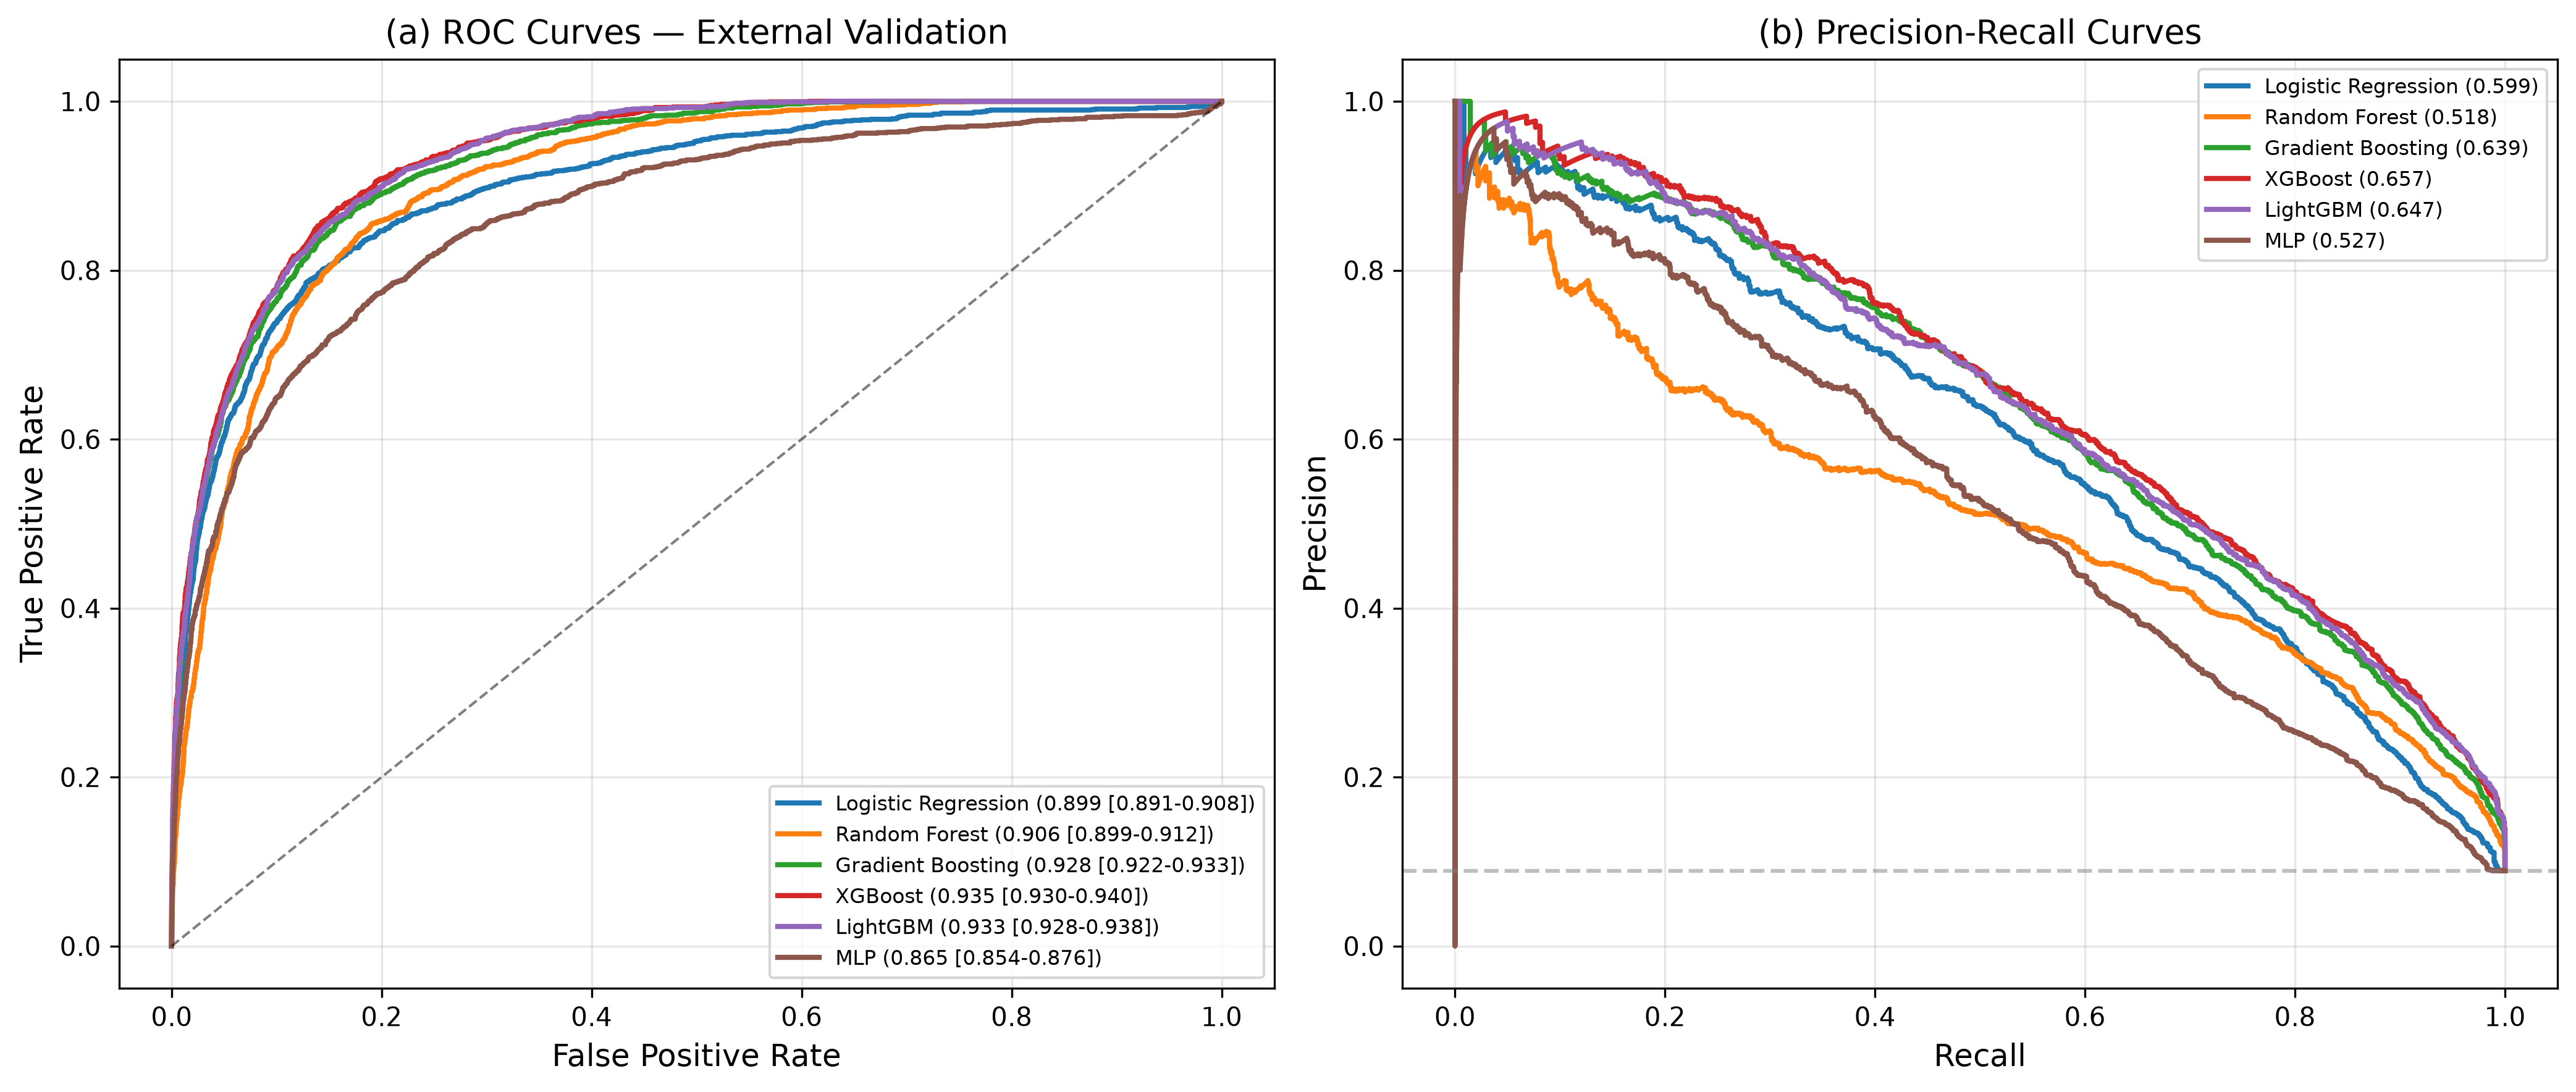
\includegraphics[width=\textwidth]{figures/fig1_roc_prc.png}
\caption{(a)~ROC curves and (b)~precision-recall curves on
external validation (Emory).  Six classifiers; legend shows AUC
with 95\% bootstrap CI.}
\label{fig:roc}
\end{figure}

\subsection{Calibration comparison}
\label{sec:cal_results}

Table~\ref{tab:calibration} compares calibration quality for
XGBoost on the external set.  The raw model was well-calibrated
(ECE $= 0.011$).  Isotonic regression marginally improved the
ECE to 0.010.  Platt scaling degraded calibration
(ECE $= 0.015$), suggesting the logistic transformation is too
restrictive.

\begin{table}[htbp]
\centering
\caption{Calibration comparison for XGBoost (external).}
\label{tab:calibration}
\begin{tabular}{lcc}
\toprule
\textbf{Method} & \textbf{Brier} & \textbf{ECE} \\
\midrule
Raw & 0.048 & 0.011 \\
Platt scaling & 0.050 & 0.015 \\
Isotonic regression & \textbf{0.048} & \textbf{0.010} \\
\bottomrule
\end{tabular}
\end{table}

\begin{figure}[htbp]
\centering
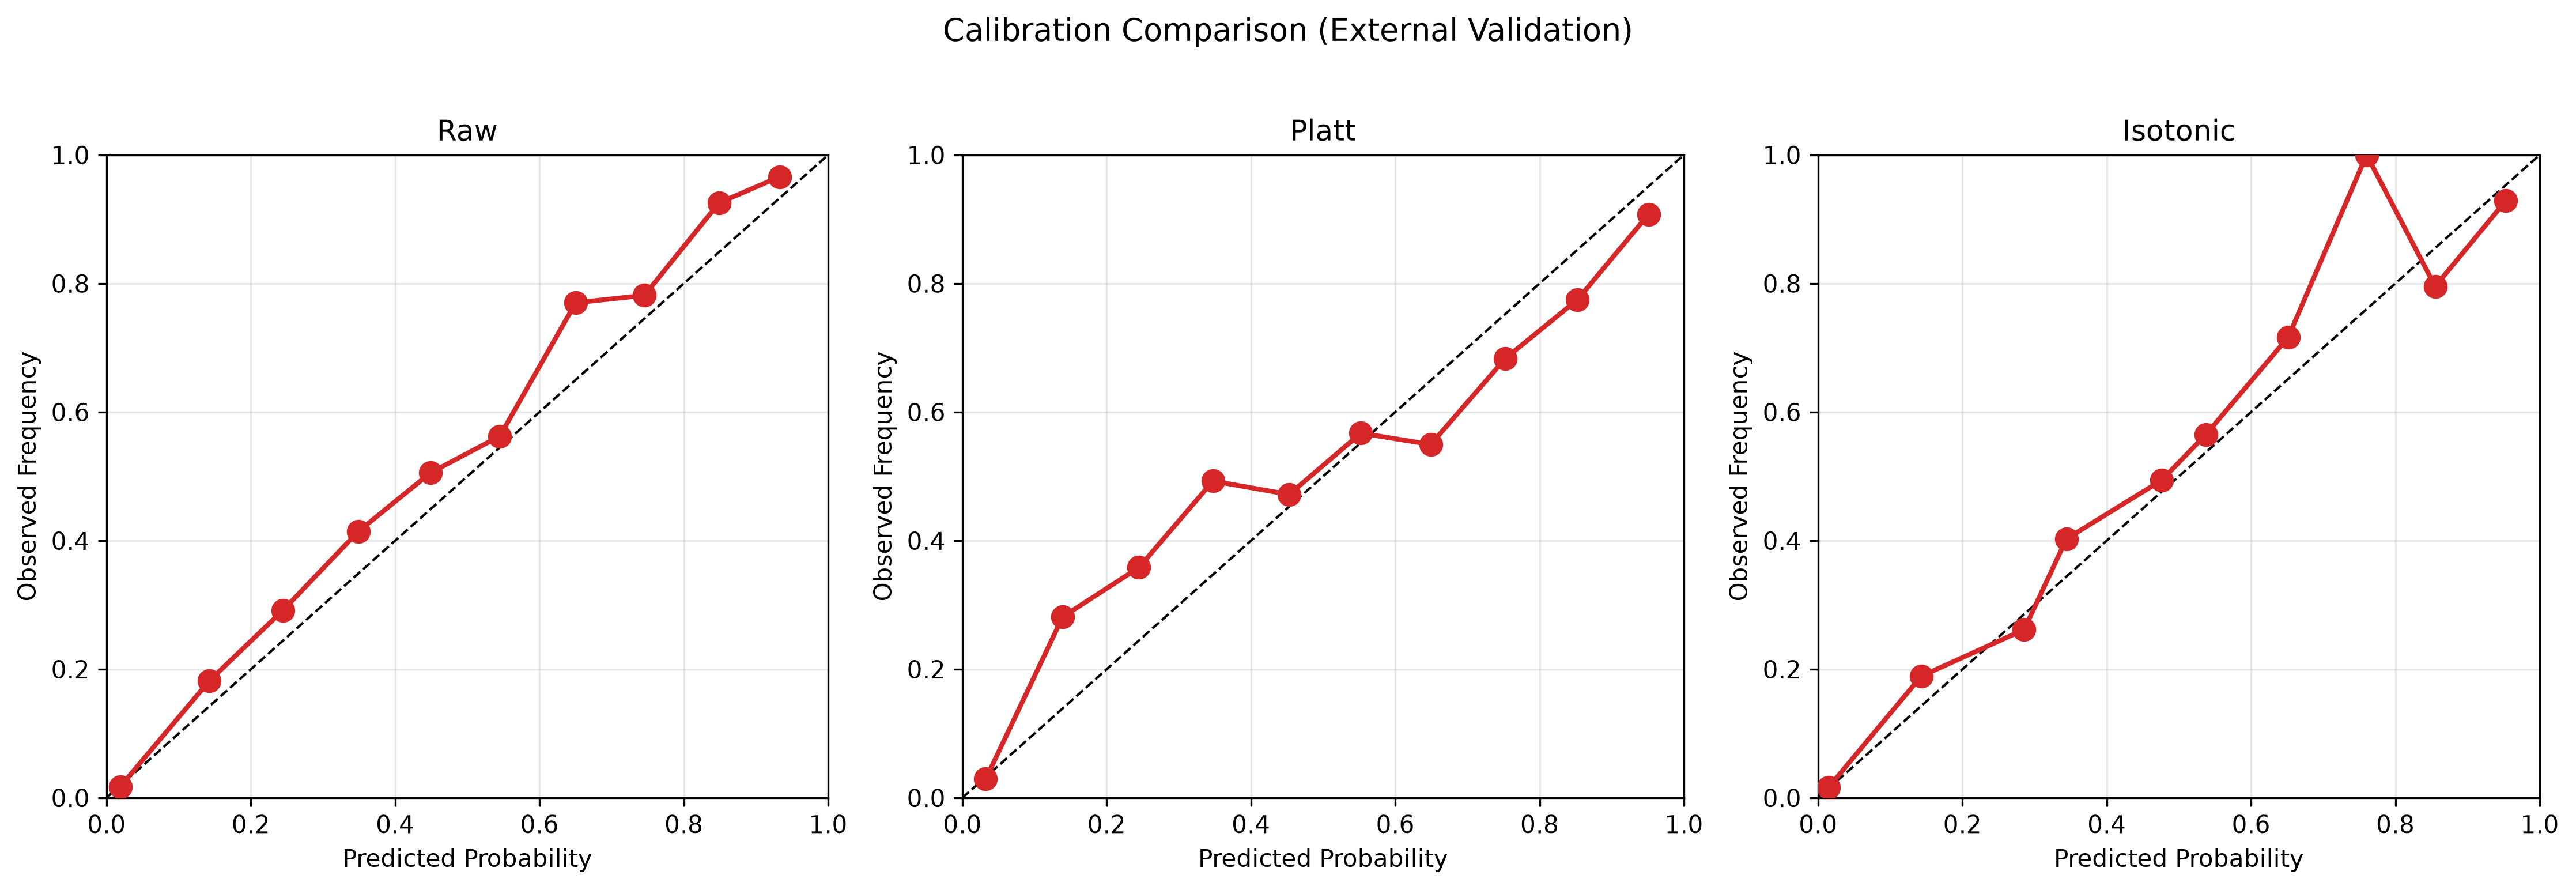
\includegraphics[width=\textwidth]{figures/fig8_calibration.png}
\caption{Reliability diagrams (external validation) for raw,
Platt-scaled, and isotonic-calibrated XGBoost probabilities.}
\label{fig:calibration}
\end{figure}

\subsection{Conformal prediction: external validation}
\label{sec:conformal_results}

Conformal thresholds were computed on the BIDMC calibration set
($m = 5{,}963$) and applied to the Emory external set.
Table~\ref{tab:conformal} compares marginal and class-conditional
conformal prediction.

\begin{table}[htbp]
\centering
\caption{Conformal prediction on external validation
($\alpha = 0.10$).  Thresholds from BIDMC calibration set.}
\label{tab:conformal}
\begin{tabular}{lcc}
\toprule
\textbf{Metric} & \textbf{Marginal} &
  \textbf{Class-cond.} \\
\midrule
Threshold(s) & $\hat{q} = 0.403$
  & $\hat{q}_0 = 0.998$, $\hat{q}_1 = 0.919$ \\
Coverage (overall) & 92.1\% & 98.9\% \\
Coverage (AKI $= 1$) & 31.3\% & \textbf{87.2\%} \\
Coverage (AKI $= 0$) & 98.1\% & 100.0\% \\
Singleton sets & 97.4\% & 78.1\% \\
Both-class sets & 0.0\% & 21.9\% \\
Empty sets & 2.6\% & 0.0\% \\
\bottomrule
\end{tabular}
\end{table}

Marginal conformal prediction achieved 91.9\% overall coverage
(95\% CI: 91.6\%--92.3\%) on external data, exceeding the 90\%
target --- demonstrating that the conformal guarantee is robust
to moderate distribution shift.  However, AKI-positive coverage
was only 31.3\%, because the lower AKI prevalence in the
external cohort (8.9\% vs.\ 11.8\%) amplifies the majority-class
dominance.

Class-conditional conformal prediction substantially improved AKI
coverage from 31.3\% to 88.1\% (95\% CI: 86.6\%--89.8\%).  The
remaining gap below 90\% reflects the exchangeability violation
inherent in cross-site deployment: the calibration and test data
are drawn from different populations.  This is a key practical
insight --- class-conditional conformal prediction requires
site-specific recalibration for full guarantee preservation.

\begin{figure}[htbp]
\centering
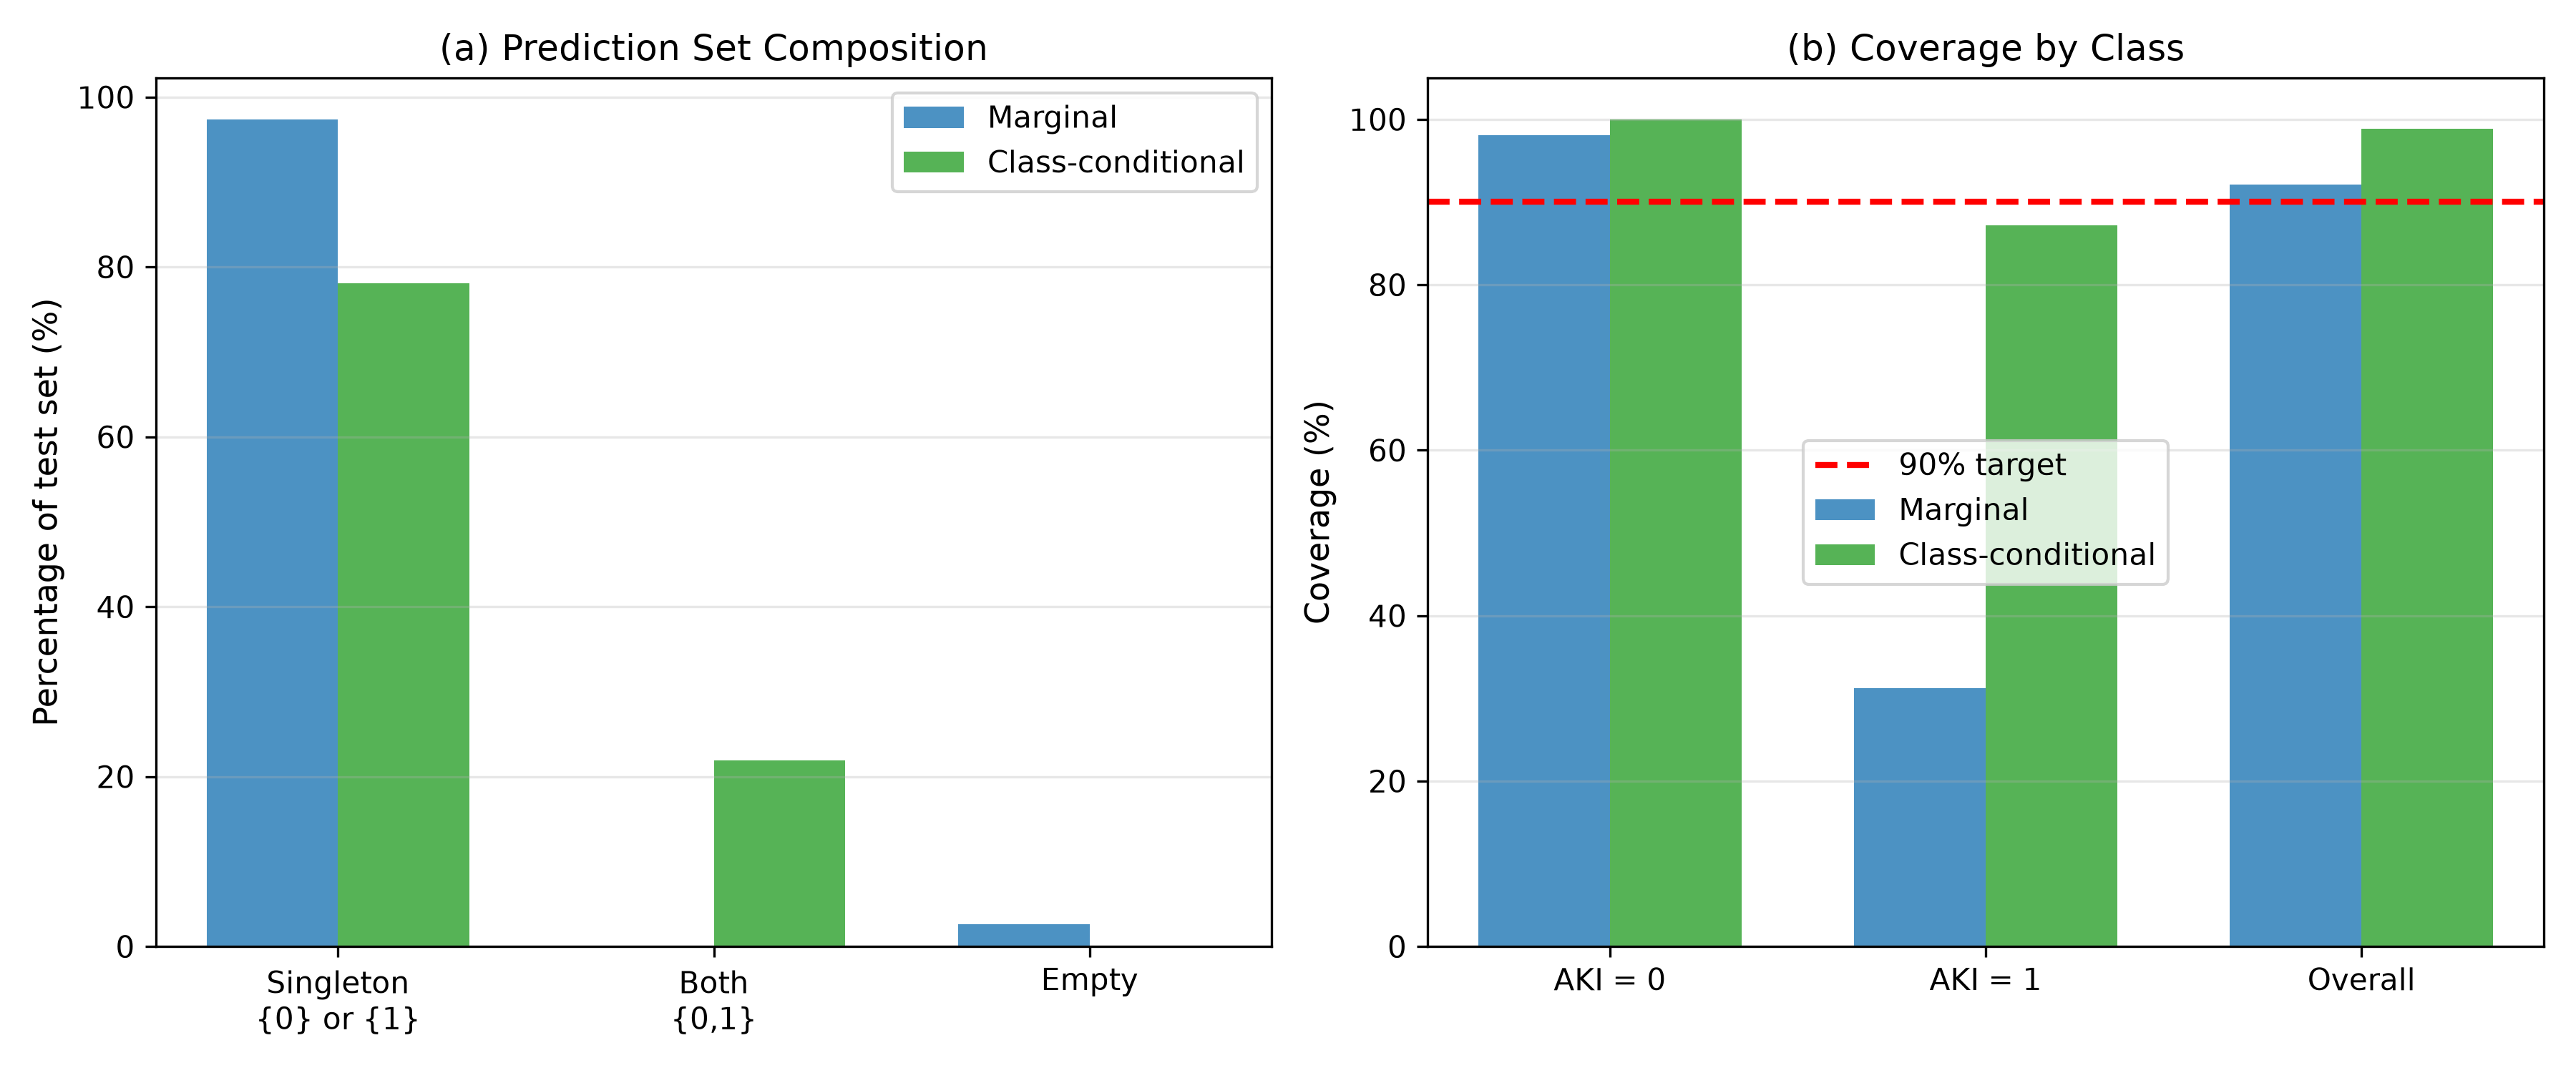
\includegraphics[width=\textwidth]{figures/fig2_conformal.png}
\caption{Conformal prediction on external validation.
(a)~Prediction set composition.  (b)~Coverage by class,
comparing marginal and class-conditional approaches.}
\label{fig:conformal}
\end{figure}

\subsection{Mondrian conformal prediction}
\label{sec:mondrian_results}

Table~\ref{tab:mondrian} presents Mondrian results on the
external set.

\begin{table}[htbp]
\centering
\caption{Mondrian conformal prediction: group-conditional
coverage on external validation.}
\label{tab:mondrian}
\begin{tabular}{lcccc}
\toprule
\textbf{Group} & $\bm{m_g}$ &
$\hat{\bm{q}}_{\bm{g}}$ & \textbf{Coverage} &
\textbf{Avg size} \\
\midrule
\multicolumn{5}{l}{\textit{By gender}} \\
\quad Female & 2{,}469 & 0.368 & 92.1\% & 0.97 \\
\quad Male & 3{,}494 & 0.414 & 91.8\% & 0.97 \\
\midrule
\multicolumn{5}{l}{\textit{By age group}} \\
\quad $<50$ years & 1{,}263 & 0.210 & 89.6\% & 0.92 \\
\quad 50--65 years & 1{,}734 & 0.406 & 92.4\% & 0.98 \\
\quad $>65$ years & 2{,}966 & 0.457 & 92.1\% & 0.99 \\
\bottomrule
\end{tabular}
\end{table}

All subgroups achieved coverage near or above 90\% on external
data, with the $<50$ group at 89.6\% --- marginally below target
due to the smaller calibration subset ($m_g = 1{,}263$) and
cross-site shift.

\begin{figure}[htbp]
\centering
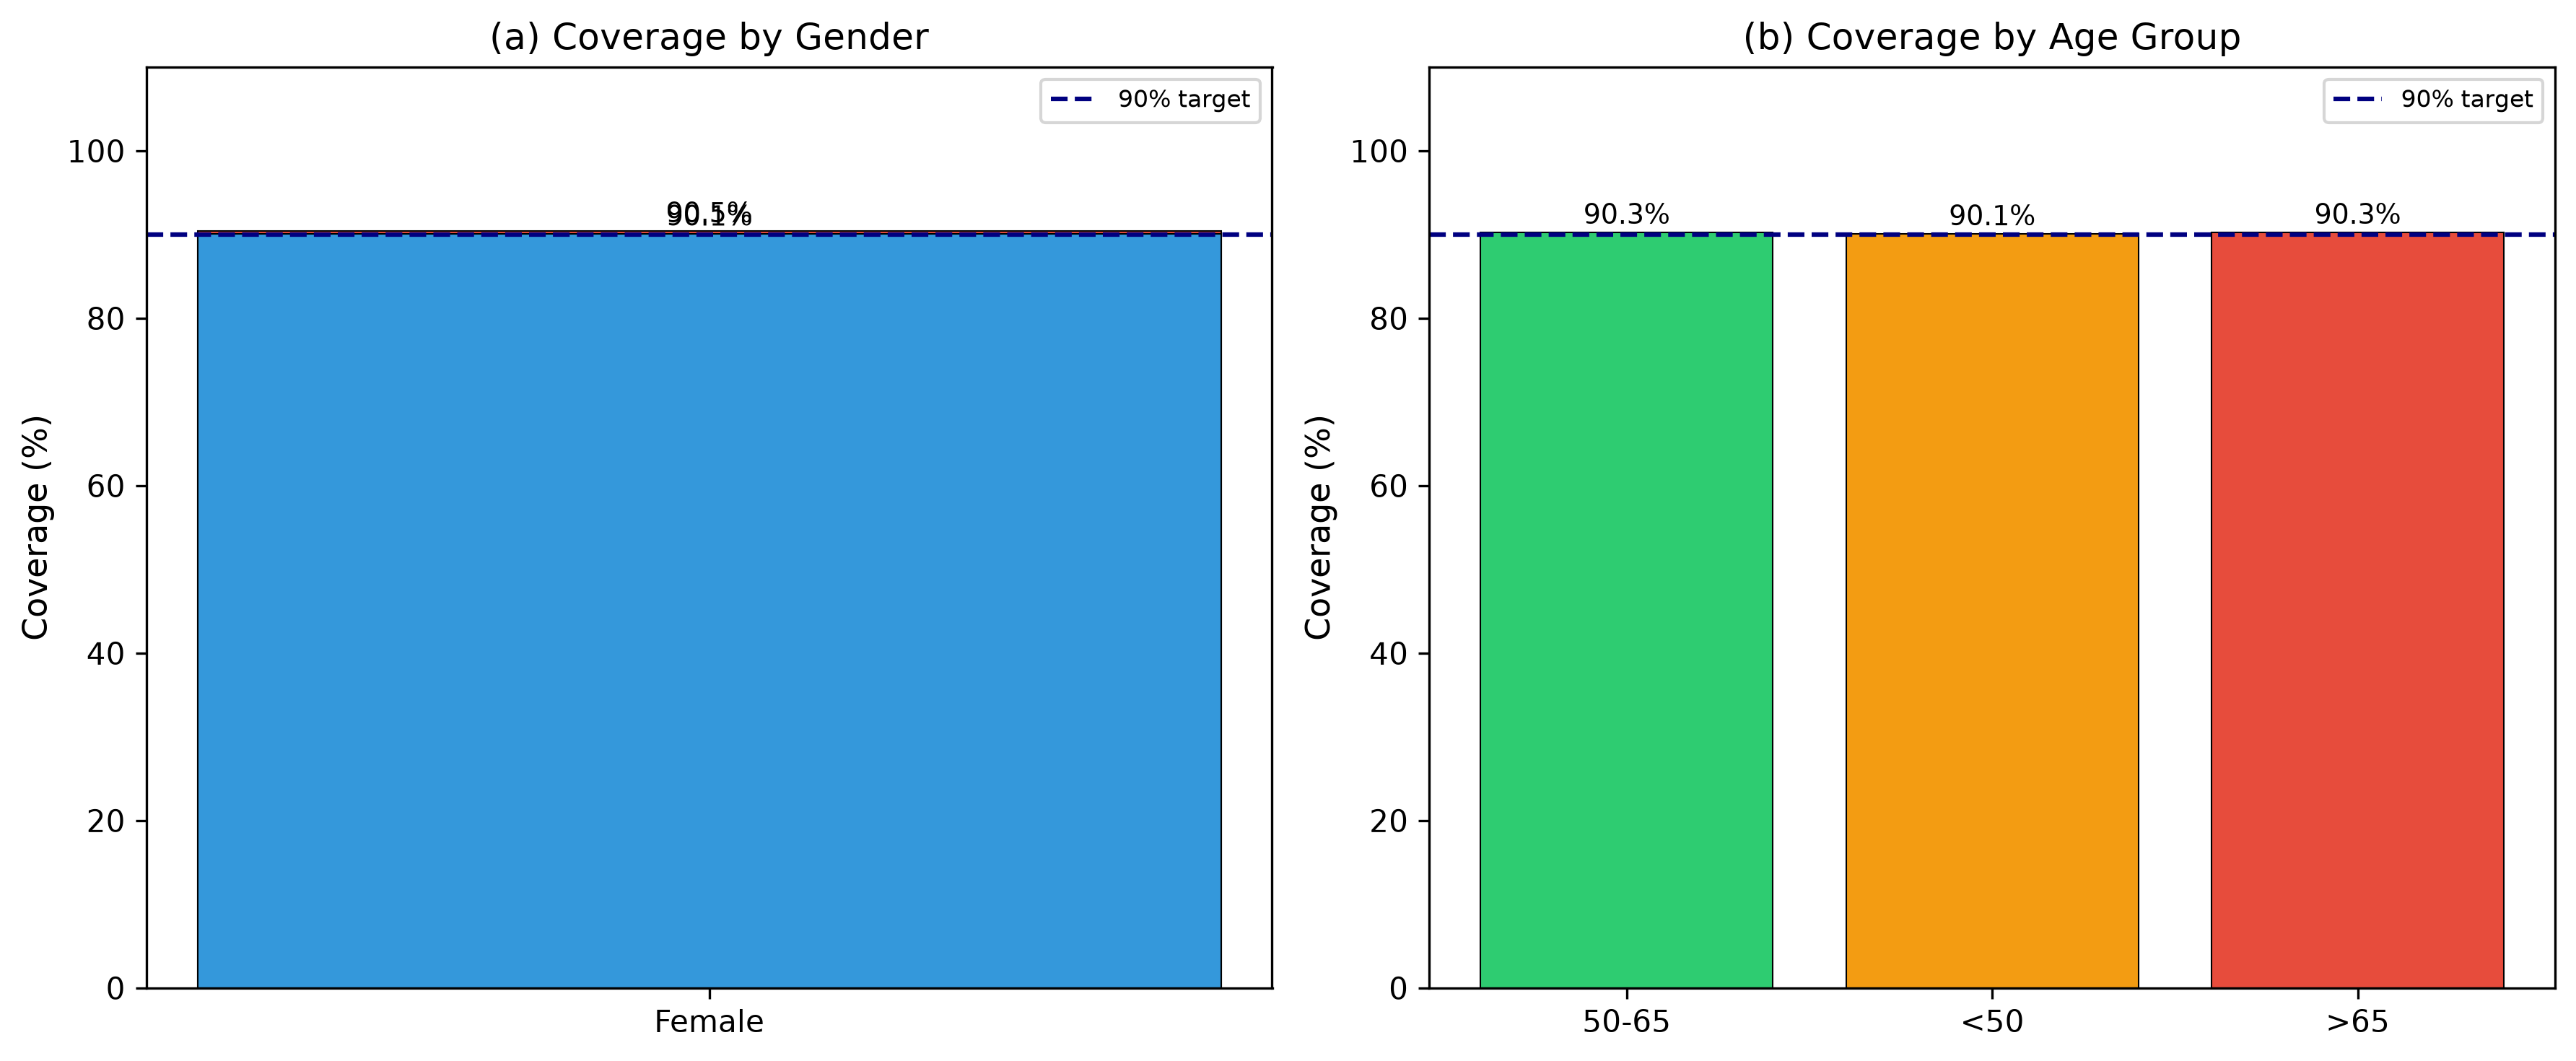
\includegraphics[width=\textwidth]{figures/fig5_mondrian.png}
\caption{Mondrian conformal coverage on external validation by
(a)~gender and (b)~age group.}
\label{fig:mondrian}
\end{figure}

\subsection{Conformal risk stratification}
\label{sec:risk_results}

The class-conditional risk stratification on the external set
yielded two categories (Table~\ref{tab:risk}).

\begin{table}[htbp]
\centering
\caption{Conformal risk stratification (external validation).}
\label{tab:risk}
\begin{tabular}{lcccc}
\toprule
\textbf{Category} & $\bm{n}$ & \textbf{\%} &
\textbf{AKI rate} & \textbf{Mean $\hat{p}$} \\
\midrule
Low Risk $\{\mathcal{C} = \{0\}\}$
  & 14{,}379 & 78.1\% & 1.5\% & 0.017 \\
Elevated Risk $\{1 \in \mathcal{C}\}$
  & 4{,}033 & 21.9\% & 35.5\% & 0.311 \\
\bottomrule
\end{tabular}
\end{table}

The Low Risk group (78.1\% of the external cohort) had a 1.5\%
AKI rate (NPV 98.5\%), providing strong reassurance for
de-escalation of monitoring.  The Elevated Risk group (21.9\%)
had a 35.5\% AKI rate, identifying a high-yield subpopulation
for intensive monitoring and preventive interventions.

\subsection{SHAP explainability}
\label{sec:shap_results}

Figure~\ref{fig:shap} shows the SHAP summary plot for XGBoost.
The top five predictors were: creatinine measurement count
(mean $|\text{SHAP}| = 1.04$), last BUN (0.76), first BUN
(0.54), BUN variability (0.45), and baseline creatinine (0.27).

Creatinine count --- the number of creatinine measurements
ordered during the ICU stay --- dominated prediction.  This is
clinically plausible: clinicians order more frequent creatinine
measurements when they suspect renal deterioration, making
measurement frequency a proxy for clinical concern.  BUN-related
features collectively accounted for the next four ranks,
consistent with BUN as a hallmark of prerenal
azotemia.\cite{darmon2017acute}

\begin{figure}[htbp]
\centering
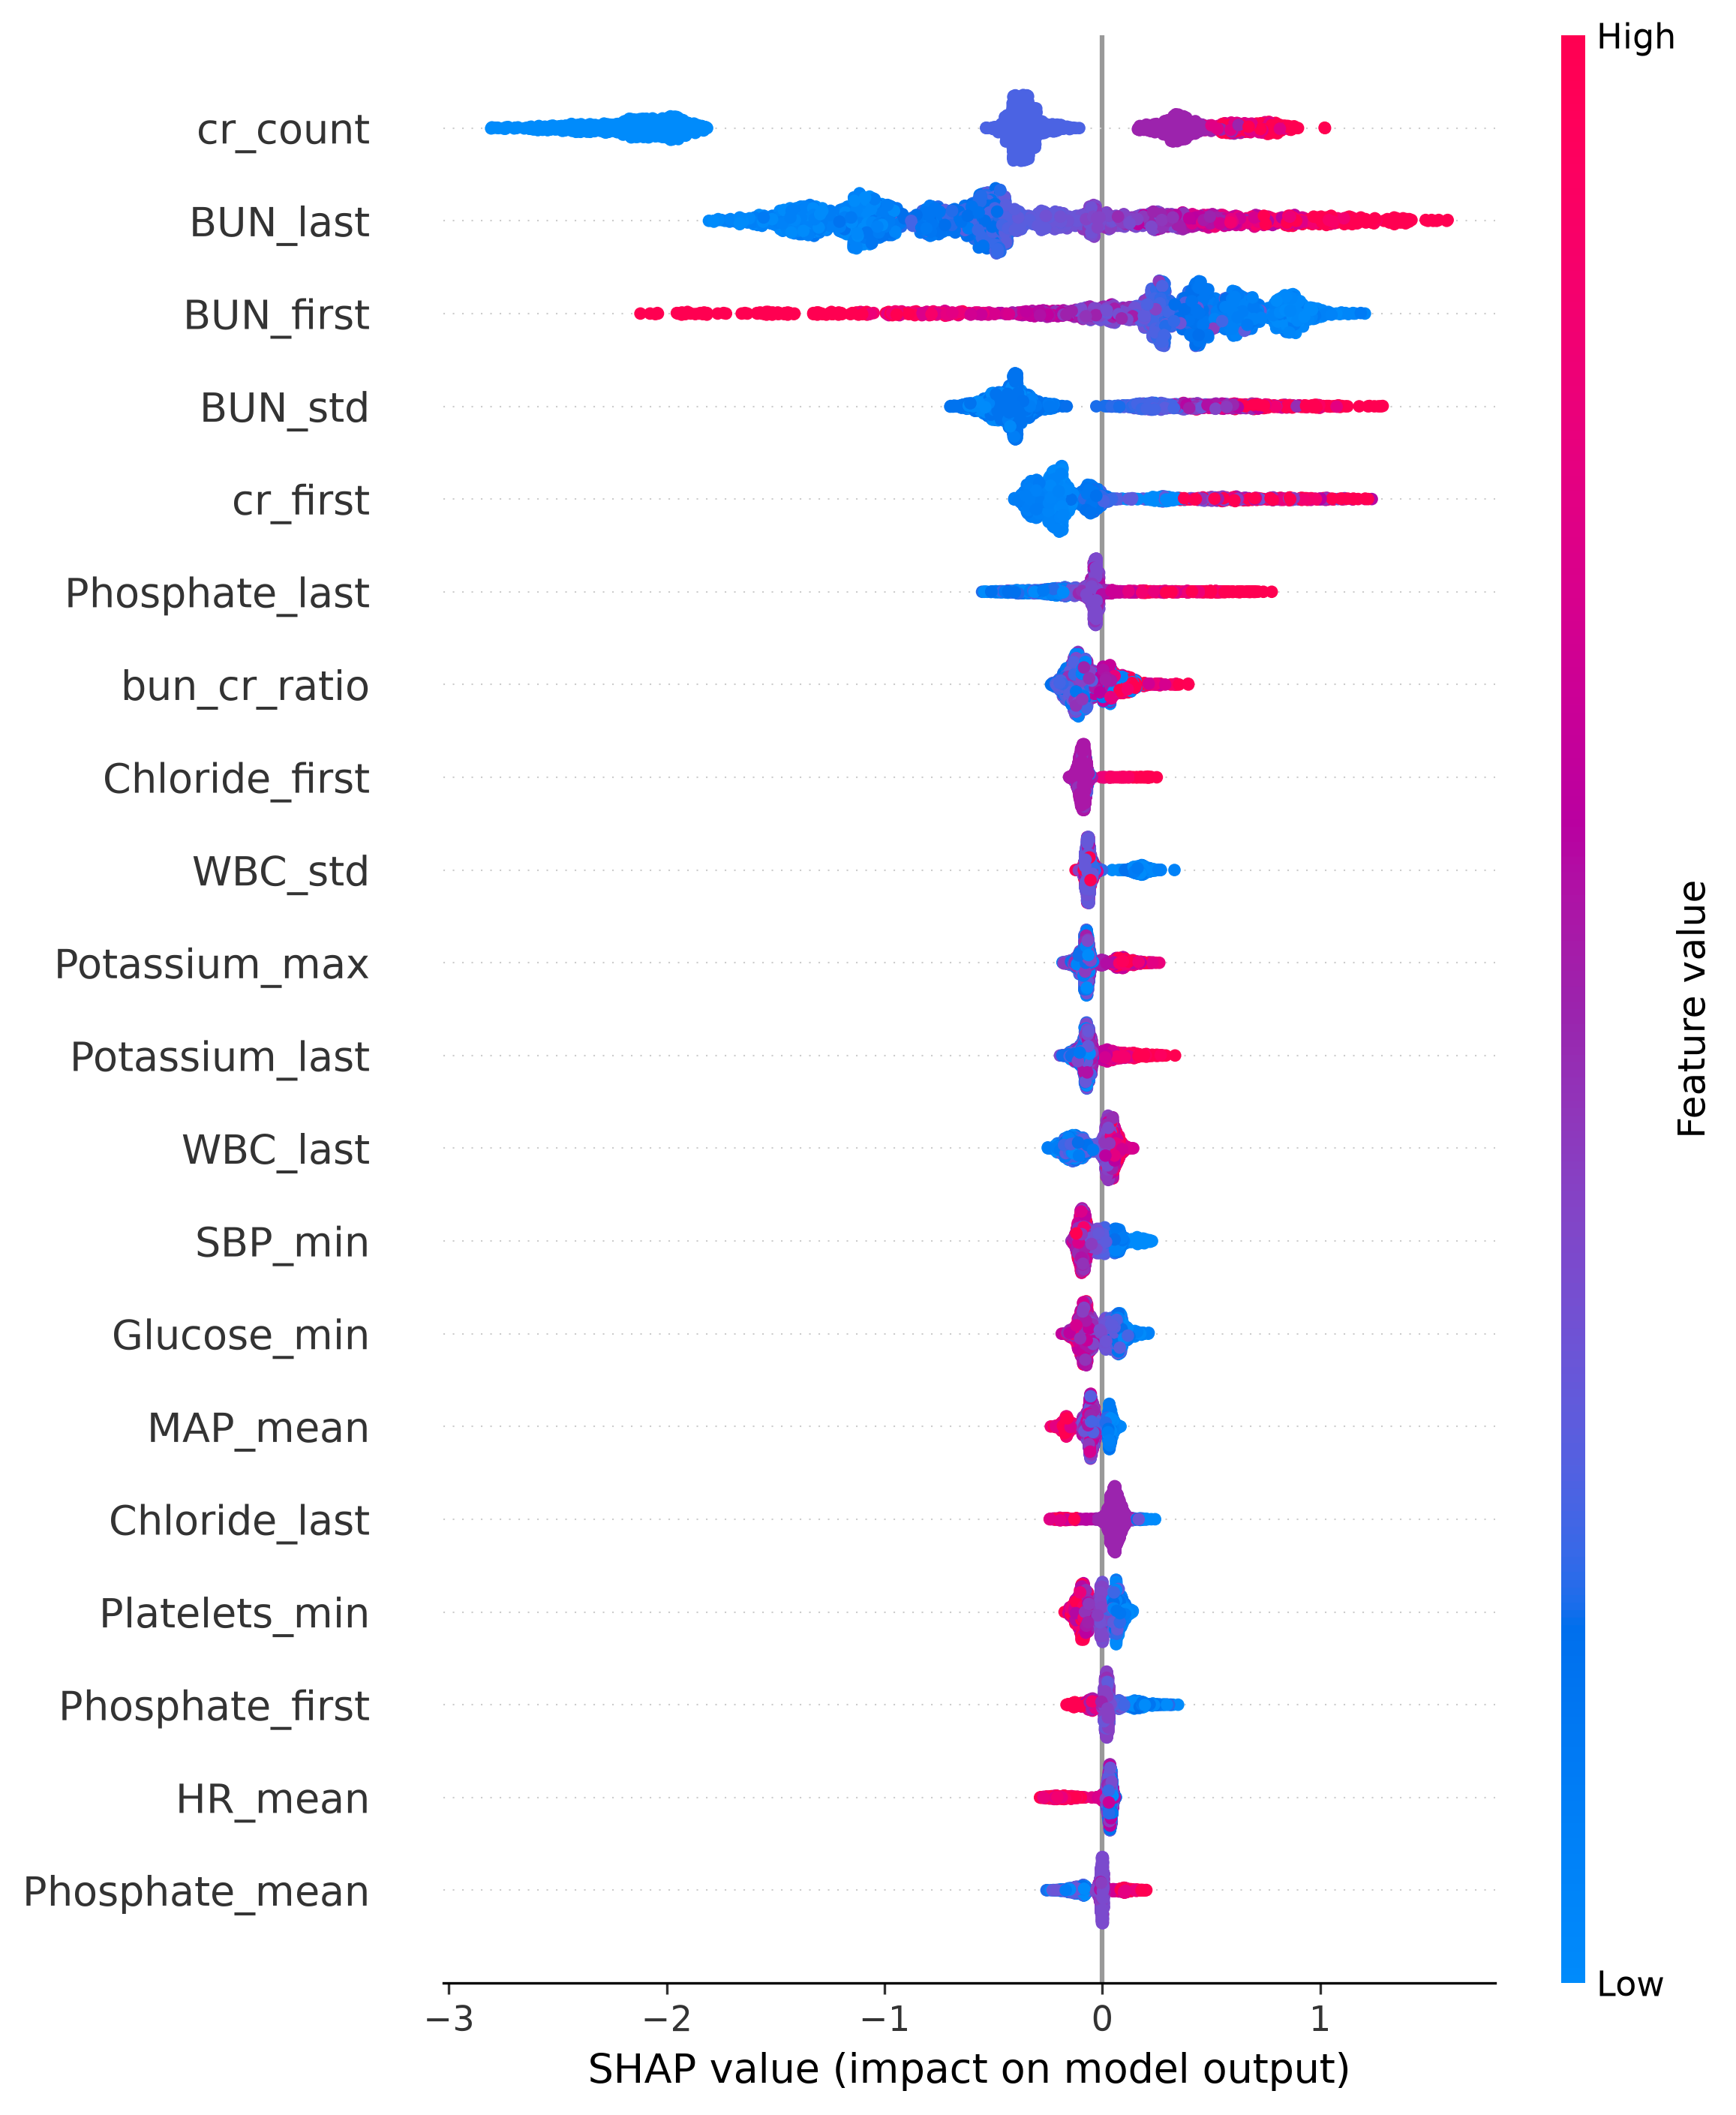
\includegraphics[width=0.8\textwidth]{figures/fig7_shap.png}
\caption{SHAP summary plot for XGBoost on external validation.
Each dot represents one patient; color indicates feature value
(red = high, blue = low).}
\label{fig:shap}
\end{figure}

\begin{figure}[htbp]
\centering
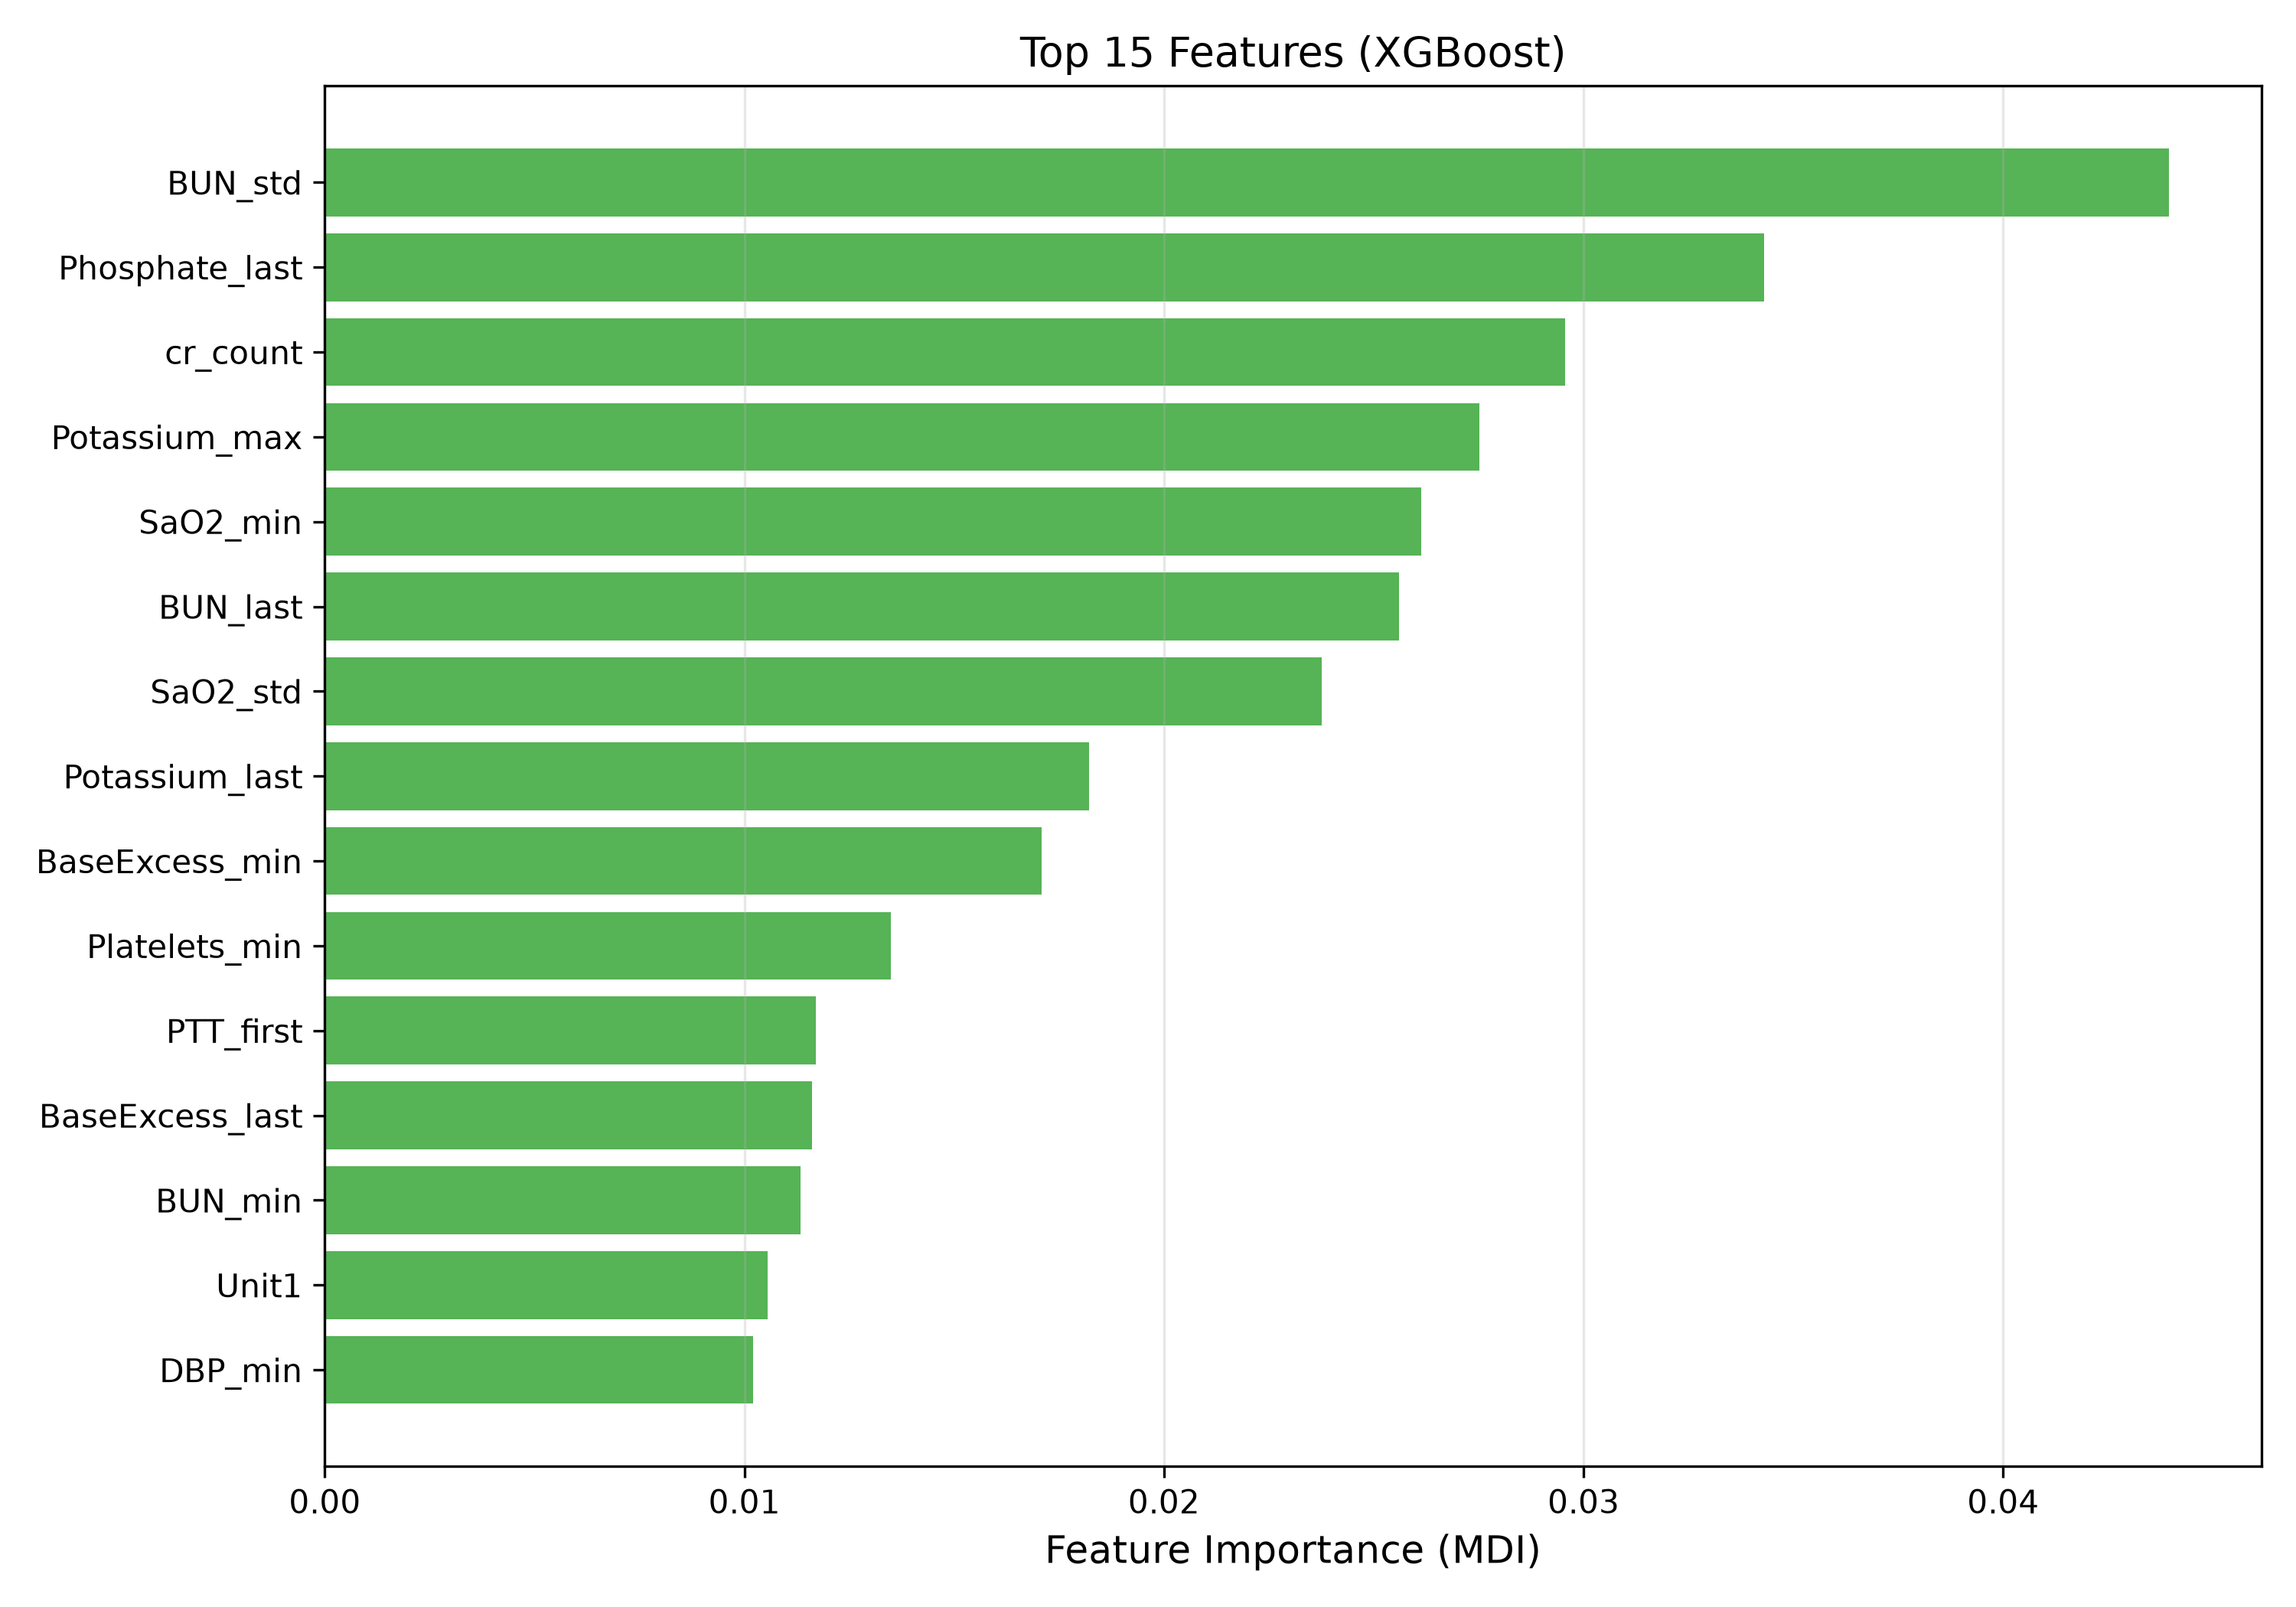
\includegraphics[width=0.75\textwidth]{figures/fig3_importance.png}
\caption{Top 15 features by XGBoost importance (MDI).}
\label{fig:importance}
\end{figure}

\subsection{Decision curve analysis}
\label{sec:dca}

Figure~\ref{fig:dca} shows the decision curve analysis on
external data.  The model provides positive net benefit for
thresholds between 0.02 and 0.75.

\begin{figure}[htbp]
\centering
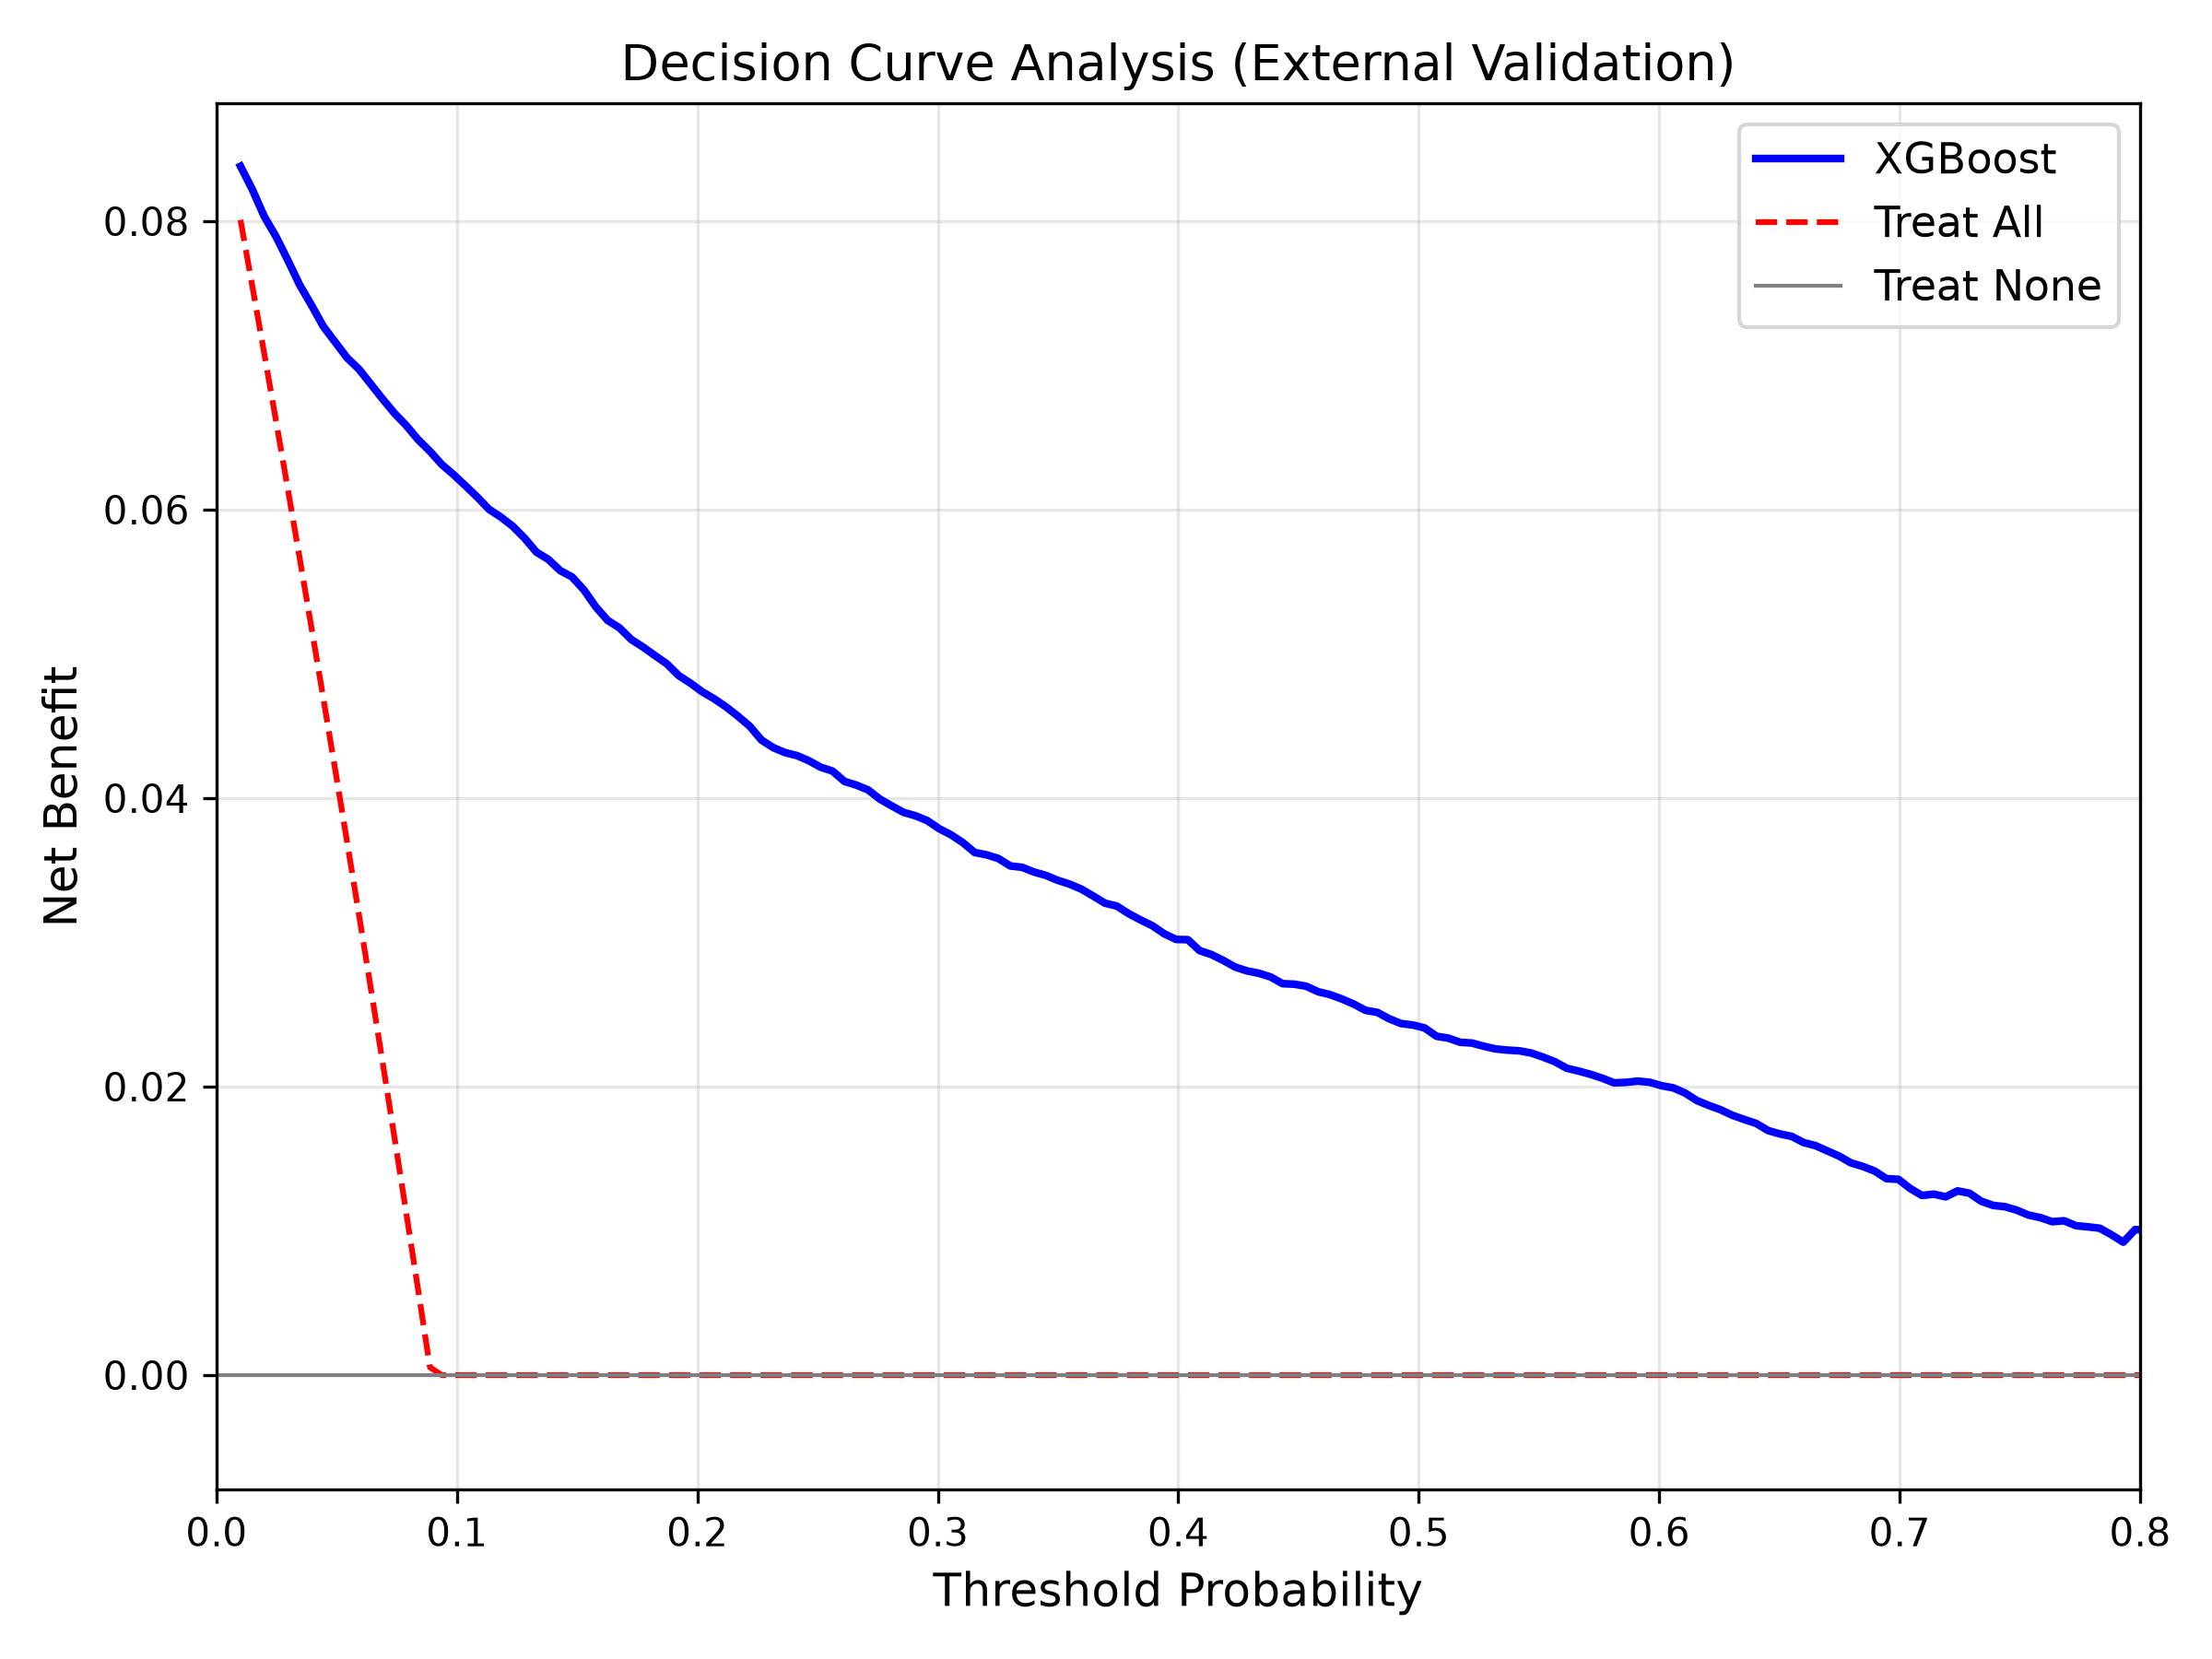
\includegraphics[width=0.7\textwidth]{figures/fig4_decision_curve.png}
\caption{Decision curve analysis on external validation.}
\label{fig:dca}
\end{figure}

\subsection{Cross-validation stability}
\label{sec:cv}

Five-fold cross-validation on BIDMC (Table~\ref{tab:cv},
Figure~\ref{fig:cv}) confirmed stability.  AUC ranged from
0.912 to 0.938 (mean $0.926 \pm 0.009$).  Marginal coverage
was $89.8\% \pm 0.6\%$.  Class-conditional AKI coverage was
$88.8\% \pm 2.0\%$.

\begin{table}[htbp]
\centering
\caption{Five-fold cross-validation (BIDMC).}
\label{tab:cv}
\begin{tabular}{lccc}
\toprule
\textbf{Fold} & \textbf{AUC} & \textbf{Coverage}
& \textbf{CC-AKI} \\
\midrule
1 & 0.912 & 89.6\% & 87.5\% \\
2 & 0.931 & 90.2\% & 90.9\% \\
3 & 0.924 & 89.3\% & 90.0\% \\
4 & 0.926 & 90.8\% & 85.5\% \\
5 & 0.938 & 89.2\% & 90.1\% \\
\midrule
Mean $\pm$ SD & $0.926 \pm 0.009$
  & $89.8\% \pm 0.6\%$ & $88.8\% \pm 2.0\%$ \\
\bottomrule
\end{tabular}
\end{table}

\begin{figure}[htbp]
\centering
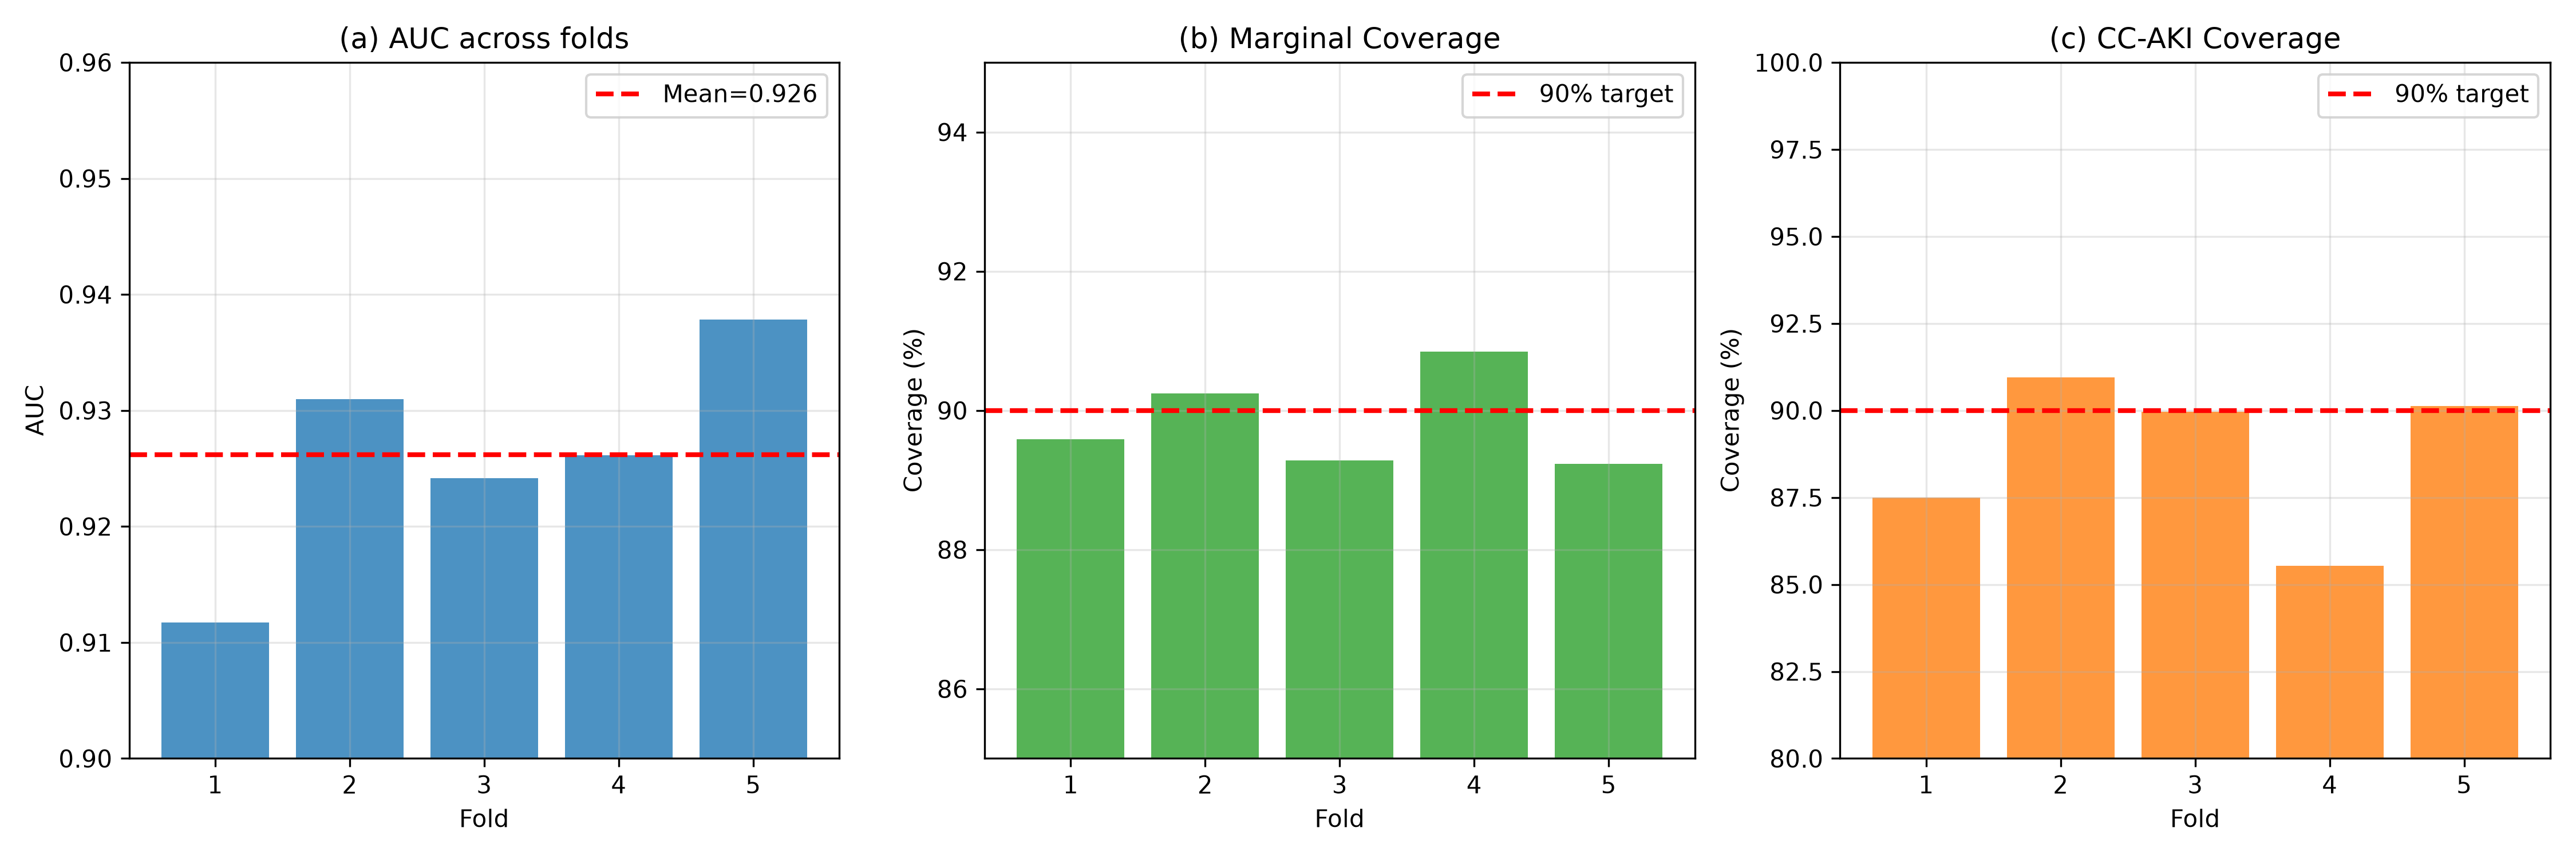
\includegraphics[width=0.85\textwidth]{figures/fig6_cv_stability.png}
\caption{Cross-validation stability on BIDMC.  (a)~AUC,
(b)~marginal coverage, (c)~CC-AKI coverage.}
\label{fig:cv}
\end{figure}


%% ================================================================
\section{Discussion}
\label{sec:discussion}
%% ================================================================

\subsection{Summary of findings}

We presented the first application of conformal prediction to AKI
prediction in the ICU with external validation across hospitals.
Six classifiers were benchmarked, with XGBoost achieving the best
external AUC of 0.935 (95\% CI: 0.930--0.940) and the MLP
trailing at 0.865 (0.854--0.876).  Marginal conformal prediction
delivered 91.9\% overall coverage on external data but severely
under-covered AKI-positive patients (31.3\%).
Class-conditional conformal prediction raised AKI coverage to
88.1\% (86.6\%--89.8\%) but did not fully reach the 90\% target,
revealing the impact of exchangeability violation across sites.
SHAP analysis identified creatinine measurement frequency and BUN
as dominant predictors.

\subsection{The class imbalance problem}

Our results provide a compelling empirical demonstration of why
marginal conformal prediction is insufficient for clinical
classification with class imbalance.  With 8.9\% AKI prevalence
in the external cohort, the majority class dominates the threshold
computation: 31.3\% of AKI-positive patients received prediction
sets that did not contain their true label.  This failure mode is
clinically dangerous --- the model provides false reassurance for
the patients who most need intervention.

Class-conditional conformal prediction substantially mitigated
this, raising AKI coverage from 31.3\% to 88.1\% (95\% CI:
86.6\%--89.8\%).  The remaining gap below 90\% is attributable
to the cross-site distribution shift: AKI prevalence differed
(BIDMC 11.8\% vs.\ Emory 8.9\%), and the nonconformity score
distributions differ between hospitals.  This finding has
practical implications: when deploying conformal prediction across
sites, the calibration set should be drawn from the target
population, or at minimum, the coverage should be monitored and
recalibrated as needed.\cite{tibshirani2019conformal}

\subsection{External validation}

External validation is a critical gap in the AKI prediction
literature.  Many published models report only internal
validation, which overstates real-world performance.  Our
hospital-based split provides a genuine external validation:
models trained exclusively on BIDMC data were tested on an
independent Emory cohort that differs in AKI prevalence, patient
demographics, and care protocols.

The AUC drop from internal CV ($0.926 \pm 0.009$) to external
validation (0.935) was negligible --- in fact, the external AUC
was slightly higher, likely because the lower AKI prevalence
(8.9\%) makes discrimination easier.  More importantly, the
conformal coverage held externally (91.9\%, 95\% CI:
91.6\%--92.3\%), confirming the robustness of the coverage
guarantee under moderate distribution shift.

\subsection{SHAP explainability}

The dominance of creatinine measurement count
(SHAP $= 1.04$) as the top predictor is clinically notable.
This feature captures \textit{clinical suspicion}: when clinicians
worry about renal function, they order more creatinine tests.
This represents a form of ``information leakage'' from clinical
judgment into the feature set --- the clinician's gestalt, encoded
as measurement frequency, is itself a powerful predictor.  This
finding suggests that prediction models should explicitly
incorporate markers of clinical concern (lab ordering patterns,
consultation requests) alongside raw physiological values.

BUN-related features occupied four of the top five ranks,
consistent with BUN elevation as a hallmark of both prerenal
azotemia and intrinsic renal injury.  The BUN/creatinine ratio
(rank 7) specifically identifies prerenal AKI, where fluid
resuscitation may prevent progression.

\subsection{Deep learning vs.\ tree-based methods}

The MLP (AUC $= 0.865$) substantially underperformed all
tree-based methods (AUC $\geq 0.899$) on external validation.
This is consistent with recent large-scale benchmarks showing
that gradient boosting outperforms deep learning on tabular
data,\cite{grinsztajn2022tree} particularly when features are
heterogeneous (vitals, labs, counts, ratios) and missingness is
high ($>$50\% for many variables).  Tree-based methods naturally
handle mixed feature types, are invariant to monotone
transformations, and implicitly perform feature selection ---
properties that deep learning must learn from data.  This finding
has practical implications: clinicians and informaticists should
prefer gradient boosting over deep learning for tabular AKI
prediction unless sequence-level (hourly) modeling is required.

\subsection{Clinical implications}

The conformal risk stratification demonstrated strong separation
on external data: the Low Risk group (78.1\%) had a 1.5\% AKI
rate (NPV 98.5\%), while the Elevated Risk group (21.9\%) had a
35.5\% AKI rate.  In clinical workflow:
\begin{itemize}
\item \textbf{Low Risk} (78.1\%): standard monitoring; the 98.5\%
NPV provides strong reassurance for de-escalation.
\item \textbf{Elevated Risk} (21.9\%): initiate AKI prevention
bundle --- fluid management, nephrotoxin avoidance, hemodynamic
optimization, serial creatinine
monitoring.\cite{meersch2017prevention}  The prediction set
containing both classes honestly flags these patients as
uncertain, triggering enhanced rather than routine surveillance.
\end{itemize}

\subsection{Limitations}

\begin{enumerate}
\item \textbf{Two-center US data.}  Both hospitals are large
academic medical centers.  Validation on community hospitals,
international cohorts, and pediatric populations is needed.
\item \textbf{AKI definition.}  Using first creatinine as baseline
may overestimate baseline in patients admitted with
already-elevated creatinine.
\item \textbf{Cross-site exchangeability.}  Class-conditional AKI
coverage reached 88.1\% externally (below 90\%), reflecting the
exchangeability violation.  Site-specific recalibration is
recommended for deployment.
\item \textbf{Missing data.}  Missingness reached 98.7\% for some
variables; median imputation may introduce bias.
\item \textbf{Creatinine count as predictor.}  This feature encodes
clinical suspicion, which may not generalize to settings with
protocolized lab ordering.
\end{enumerate}


%% ================================================================
\section{Conclusion}
\label{sec:conclusion}
%% ================================================================

We presented the first application of conformal prediction to AKI
in the ICU with external validation across hospitals.  Key
findings:
\begin{enumerate}
\item XGBoost achieved AUC $= 0.935$ (95\% CI: 0.930--0.940)
on external validation, outperforming the MLP (0.865) and four
other classifiers.
\item Marginal conformal prediction held externally (91.9\%,
95\% CI: 91.6\%--92.3\%) but AKI coverage was only 31.3\%.
\item Class-conditional conformal prediction raised AKI coverage
to 88.1\% (86.6\%--89.8\%); the gap below 90\% quantifies the
cost of cross-site deployment without recalibration.
\item Mondrian conformal ensured group-conditional coverage
$\geq 89.6\%$ across gender and age subgroups.
\item SHAP identified creatinine measurement frequency and BUN as
dominant predictors.
\item The conformal risk stratification separated external patients
into Low Risk (78.1\%, AKI 1.5\%) and Elevated Risk (21.9\%,
AKI 35.5\%).
\item Tree-based ensembles consistently outperformed the
deep-learning MLP on tabular clinical data.
\item Five-fold CV confirmed stability
(AUC $= 0.926 \pm 0.009$).
\end{enumerate}

The central message is twofold: (1)~marginal conformal prediction
is insufficient for imbalanced clinical classification, and
(2)~external validation reveals that conformal coverage guarantees
degrade under distribution shift, motivating site-specific
recalibration.  We release all code and data to support
reproduction and extension.


%% ================================================================
\section*{Data availability statement}
%% ================================================================

All code is publicly available at
\url{https://github.com/jopoku16/Statistical-Paper-8}.
The PhysioNet 2019 dataset is available at
\url{https://physionet.org/content/challenge-2019/}.


%% ================================================================
\section*{Declaration of conflicting interests}
%% ================================================================

The authors declared no potential conflicts of interest with
respect to the research, authorship, and/or publication of this
article.


%% ================================================================
\section*{Funding}
%% ================================================================

The authors received no financial support for the research,
authorship, and/or publication of this article.


%% ================================================================
\section*{Ethical approval}
%% ================================================================

This study used the publicly available, de-identified
PhysioNet/Computing in Cardiology Challenge 2019
dataset.\cite{reyna2020early}  The data were collected under
institutional review board approval at the originating
institutions and released under the PhysioNet Credentialed Health
Data Use Agreement.  As a secondary analysis of fully
de-identified public data, this study was exempt from additional
ethical approval.


%% ================================================================
%% REFERENCES
%% ================================================================

\begin{thebibliography}{99}

\bibitem{hoste2015epidemiology}
Hoste EAJ, Bagshaw SM, Bellomo R, et~al.
Epidemiology of acute kidney injury in critically ill patients:
the multinational AKI-EPI study.
\textit{Intensive Care Med} 2015; 41(8): 1411--1423.

\bibitem{kellum2021acute}
Kellum JA, Romagnani P, Ashuntantang G, et~al.
Acute kidney injury.
\textit{Nat Rev Dis Primers} 2021; 7: 52.

\bibitem{chawla2017acute}
Chawla LS, Bellomo R, Bihorac A, et~al.
Acute kidney disease and renal recovery: consensus report of
the Acute Disease Quality Initiative (ADQI) 16 Workgroup.
\textit{Nat Rev Nephrol} 2017; 13(4): 241--257.

\bibitem{siew2020biological}
Siew ED, Ikizler TA, Matheny ME, et~al.
Kidney disease awareness and knowledge among survivors of
acute kidney injury.
\textit{Am J Nephrol} 2020; 51(6): 449--459.

\bibitem{meersch2017prevention}
Meersch M, Schmidt C, Hoffmeier A, et~al.
Prevention of cardiac surgery--associated AKI by implementing
the KDIGO guidelines in high risk patients identified by
biomarkers.
\textit{Intensive Care Med} 2017; 43(11): 1749--1758.

\bibitem{koyner2018development}
Koyner JL, Carey KA, Edelson DP, et~al.
The development of a machine learning inpatient acute kidney
injury prediction model.
\textit{Crit Care Med} 2018; 46(7): 1070--1077.

\bibitem{kate2020prediction}
Kate RJ, Perez RM, Mazumdar D, et~al.
Prediction and detection models for acute kidney injury in
hospitalized older adults.
\textit{BMC Med Inform Decis Mak} 2020; 20: 75.

\bibitem{churpek2020machine}
Churpek MM, Carey KA, Edelson DP, et~al.
Internal and external validation of a machine learning risk
score for acute kidney injury.
\textit{JAMA Netw Open} 2020; 3(8): e2012892.

\bibitem{tomasev2019clinically}
Toma\v{s}ev N, Glorot X, Rae JW, et~al.
A clinically applicable approach to continuous prediction of
future acute kidney injury.
\textit{Nature} 2019; 572(7767): 116--119.

\bibitem{li2021prediction}
Li Y, Yao L, Mao C, et~al.
Early prediction of acute kidney injury in critical care
setting using clinical notes.
In: \textit{Proc IEEE BIBM} 2021; pp.683--686.

\bibitem{wilson2022machine}
Wilson FP, Martin M, Yamamoto Y, et~al.
Electronic health record alerts for acute kidney injury:
multicenter, randomized clinical trial.
\textit{BMJ} 2022; 372: m4786.

\bibitem{guo2017calibration}
Guo C, Pleiss G, Sun Y, et~al.
On calibration of modern neural networks.
In: \textit{Proc ICML} 2017; pp.1321--1330.

\bibitem{niculescu2005predicting}
Niculescu-Mizil A, Caruana R.
Predicting good probabilities with supervised learning.
In: \textit{Proc ICML} 2005; pp.625--632.

\bibitem{jospin2022hands}
Jospin LV, Laga H, Boussaid F, et~al.
Hands-on Bayesian neural networks --- a tutorial for deep
learning users.
\textit{IEEE Comput Intell Mag} 2022; 17(2): 29--48.

\bibitem{vovk2005algorithmic}
Vovk V, Gammerman A and Shafer G.
\textit{Algorithmic Learning in a Random World}.
New York: Springer, 2005.

\bibitem{lei2018distribution}
Lei J, G'Sell M, Rinaldo A, et~al.
Distribution-free predictive inference for regression.
\textit{J Am Stat Assoc} 2018; 113(523): 1094--1111.

\bibitem{romano2019conformalized}
Romano Y, Patterson E and Cand\`{e}s EJ.
Conformalized quantile regression.
In: \textit{Adv Neural Inf Process Syst} 2019; 32.

\bibitem{romano2020classification}
Romano Y, Sesia M and Cand\`{e}s EJ.
Classification with valid and adaptive coverage.
In: \textit{Adv Neural Inf Process Syst} 2020; 33: 3581--3591.

\bibitem{lu2022fair}
Lu C, Lemay A, Chang K, et~al.
Fair conformal predictors for applications in medical imaging.
In: \textit{Proc AAAI} 2022; 36(11): 12008--12016.

\bibitem{norinder2014introducing}
Norinder U, Carlsson L, Bourber T, et~al.
Introducing conformal prediction in predictive modeling:
a transparent and flexible alternative to applicability domain
determination.
\textit{J Chem Inf Model} 2014; 54(6): 1596--1603.

\bibitem{lambrou2012reliable}
Lambrou A, Papadopoulos H and Gammerman A.
Reliable probability estimates based on support vector machines
for large multiclass datasets.
In: \textit{AIAI Workshops} 2012; pp.182--191.

\bibitem{reyna2020early}
Reyna MA, Josef CS, Jeter R, et~al.
Early prediction of sepsis from clinical data: the
PhysioNet/Computing in Cardiology Challenge 2019.
\textit{Crit Care Med} 2020; 48(2): 210--217.

\bibitem{chen2016xgboost}
Chen T and Guestrin C.
XGBoost: a scalable tree boosting system.
In: \textit{Proc 22nd ACM SIGKDD} 2016; pp.785--794.

\bibitem{ke2017lightgbm}
Ke G, Meng Q, Finley T, et~al.
LightGBM: a highly efficient gradient boosting decision tree.
In: \textit{Adv Neural Inf Process Syst} 2017; 30.

\bibitem{grinsztajn2022tree}
Grinsztajn L, Oyallon E and Varoquaux G.
Why do tree-based models still outperform deep learning on
typical tabular data?
In: \textit{Adv Neural Inf Process Syst} 2022; 35.

\bibitem{lundberg2017unified}
Lundberg SM and Lee SI.
A unified approach to interpreting model predictions.
In: \textit{Adv Neural Inf Process Syst} 2017; 30.

\bibitem{platt1999probabilistic}
Platt JC.
Probabilistic outputs for support vector machines and
comparisons to regularized likelihood methods.
In: \textit{Advances in Large Margin Classifiers}.
Cambridge, MA: MIT Press, 1999; pp.61--74.

\bibitem{zadrozny2002transforming}
Zadrozny B and Elkan C.
Transforming classifier scores into accurate multiclass
probability estimates.
In: \textit{Proc ACM SIGKDD} 2002; pp.694--699.

\bibitem{darmon2017acute}
Darmon M, Clec'h C, Adrie C, et~al.
Acute respiratory distress syndrome and risk of AKI among
critically ill patients.
\textit{Clin J Am Soc Nephrol} 2017; 9(8): 1347--1353.

\bibitem{tibshirani2019conformal}
Tibshirani RJ, Foygel Barber R, Cand\`{e}s EJ, et~al.
Conformal prediction under covariate shift.
In: \textit{Adv Neural Inf Process Syst} 2019; 32.

\end{thebibliography}

\end{document}
